%%%%%%%%%%%%%%%%%%%%%%%%%%%%%%%%%%%%%%%%%
% Masters/Doctoral Thesis 
% LaTeX Template
% Version 1.41 (9/9/13)
%
% This template has been downloaded from:
% http://www.latextemplates.com
%
% Original authors:
% Steven Gunn 
% http://users.ecs.soton.ac.uk/srg/softwaretools/document/templates/
% and
% Sunil Patel
% http://www.sunilpatel.co.uk/thesis-template/
%
% License:
% CC BY-NC-SA 3.0 (http://creativecommons.org/licenses/by-nc-sa/3.0/)
%
% Note:
% Make sure to edit document variables in the Thesis.cls file
%
%%%%%%%%%%%%%%%%%%%%%%%%%%%%%%%%%%%%%%%%%

%----------------------------------------------------------------------------------------
%	PACKAGES AND OTHER DOCUMENT CONFIGURATIONS
%----------------------------------------------------------------------------------------
\documentclass[11pt, a4paper, oneside]{Thesis} % Paper size, default font size and one-sided paper

\graphicspath{{Pictures/}} % Specifies the directory where pictures are stored

%\renewcommand*\listfigurename{Elenco delle figure}


\usepackage[square, numbers, comma, sort&compress]{natbib} % Use the natbib reference package - read up on this to edit the reference style; if you want text (e.g. Smith et al., 2012) for the in-text references (instead of numbers), remove 'numbers' 
\hypersetup{urlcolor=blue, colorlinks=true} % Colors hyperlinks in blue - change to black if annoying
\title{\ttitle} % Defines the thesis title - don't touch this

\usepackage[italian]{babel}
%\usepackage[]{tocbibind}
\usepackage[nottoc]{tocbibind} 
\begin{document}

%\setmarginsrb{40mm}{15mm}{40mm}{15mm}%{left}{top}{right}{bottom}
%                      {0mm}{10mm}{0mm}{10mm}  %{headheight}{headsep}{footheight}{footskip}

\frontmatter % Use roman page numbering style (i, ii, iii, iv...) for the pre-content pages

\setstretch{1.3} % Line spacing of 1.3

% Define the page headers using the FancyHdr package and set up for one-sided printing
\fancyhead{} % Clears all page headers and footers
\rhead{\thepage} % Sets the right side header to show the page number
\lhead{} % Clears the left side page header

\pagestyle{fancy} % Finally, use the "fancy" page style to implement the FancyHdr headers

\newcommand{\HRule}{\rule{\linewidth}{0.5mm}} % New command to make the lines in the title page

% PDF meta-data
\hypersetup{pdftitle={\ttitle}}
\hypersetup{pdfsubject=\subjectname}
\hypersetup{pdfauthor=\authornames}
\hypersetup{pdfkeywords=\keywordnames}

%----------------------------------------------------------------------------------------
%	TITLE PAGE
%----------------------------------------------------------------------------------------

\begin{titlepage}
\begin{center}
\HRule \\[0.4cm] % Horizontal line

\textsc{\LARGE  }\\[1.5cm] % University name

{\huge \bfseries Simulatore F1}\\[1.5cm] % Thesis title

\textsc{Progetto per il corso di Sistemi \\Concorrenti e Distribuiti}\\[0.5cm] % Thesis type

\textsc{\LARGE  }\\[1.5cm] % University name

\textsc{Settembre 2013}\\[4cm] % Date

\textsc{\LARGE  }\\[1.5cm] % University name

\begin{minipage}{0.4\textwidth}
\begin{flushleft} \large
\emph{Autori:}\\
{Claudio Guarisco - 1057761 \\} % Author name - remove the \href bracket to remove the link
{Michele Massaro - 1057513}
\end{flushleft}
\end{minipage}
\begin{minipage}{0.4\textwidth}
\begin{flushright} \large
%\emph{Supervisor:} \\
%\href{http://www.jamessmith.com}{\supname} % Supervisor name - remove the \href bracket to remove the link  
\end{flushright}
\end{minipage}\\[3cm]

\textsc{\LARGE  }\\[1.5cm] % University name

\HRule \\[1.5cm] % Horizontal line



 

 
%\large \textit{A thesis submitted in fulfilment of the requirements\\ for the degree of \degreename}\\[0.3cm] % University requirement text
%\textit{in the}\\[0.4cm]
%\groupname\\\deptname\\[2cm] % Research group name and department name
 

%\includegraphics{Logo} % University/department logo - uncomment to place it
 
\vfill
\end{center}

\end{titlepage}

%----------------------------------------------------------------------------------------
%	LIST OF CONTENTS/FIGURES/TABLES PAGES
%----------------------------------------------------------------------------------------

\pagestyle{fancy} % The page style headers have been "empty" all this time, now use the "fancy" headers as defined before to bring them back

\lhead{\emph{Indice}} % Set the left side page header to "Contents"

\tableofcontents % Write out the Table of Contents

%\lhead{\emph{Elenco delle figure}} % Set the left side page header to "List of Figures"
\listoffigures % Write out the List of Figures

%\lhead{\emph{List of Tables}} % Set the left side page header to "List of Tables"
%\listoftables % Write out the List of Tables


%----------------------------------------------------------------------------------------
%	THESIS CONTENT - CHAPTERS
%----------------------------------------------------------------------------------------

\mainmatter % Begin numeric (1,2,3...) page numbering

\pagestyle{fancy} % Return the page headers back to the "fancy" style

% Include the chapters of the thesis as separate files from the Chapters folder
% Uncomment the lines as you write the chapters

\chapter{Introduzione} % Main chapter title

\label{Chapter1} % Change X to a consecutive number; for referencing this chapter elsewhere, use \ref{ChapterX}

\lhead{Capitolo 1. \emph{Introduzione}} % Change X to a consecutive number; this is for the header on each page - perhaps a shortened title

Questo documento contiene la relazione finale del progetto di Sistemi Concorrenti e Distribuiti, riguardante la progettazione e realizzazione di un simulatore concorrente e distribuito di una competizione sportiva assimilabile a quelle automobilistiche di Formula 1.
I requisiti del sistema sono i seguenti:
\begin{itemize}
 \item un circuito, possibilmente selezionabile in fase di configurazione, dotato almeno della pista e della corsia di rifornimento, ciascuna della quali soggette a regole congruenti di accesso, condivisione, tempo di percorrenza, condizioni atmosferiche, ecc.
 \item un insieme configurabile di concorrenti, ciascuno con caratteristiche specifiche di prestazione, risorse, strategia di gara, ecc.
 \item un sistema di controllo capace di riportare costantemente, consistentemente e separatamente, lo stato della competizione, le migliori prestazioni (sul giro, per sezione di circuito) e anche la situazione di ciascun concorrente rispetto a specifici parametri tecnici
 \item una particolare competizione, con specifica configurabile della durata e controllo di terminazione dei concorrenti a fine gara.
\end{itemize}


\chapter{Problematiche} % Main chapter title

\label{Chapter2} % Change X to a consecutive number; for referencing this chapter elsewhere, use \ref{ChapterX}

\lhead{Capitolo 2. \emph{Problematiche}} % Change X to a consecutive number; this is for the header on each page - perhaps a shortened title

%----------------------------------------------------------------------------------------
%	SECTION 1
%----------------------------------------------------------------------------------------

\section{Scelta del tipo di simulazione}

I tipi di simulazioni possibili possono dividersi in due categorie:
\begin{itemize}
 \item \textbf{Continua}: può essere rappresentata come una grande macchina a stati, in cui lo stato avanza solo quando tutte le operazioni correnti vengono completate. Vengono rappresentati tutti gli stati possibili. Spesso non è possibile garantire l'avanzamento a tempo reale perchè il tick di progressione richiede un tempo maggiore del periodo temporale rappresentato, in quanto l'aggiornamento di stato richiede di considerare un numero di variabili molto elevato.
 \item \textbf{Discreta}: l’avanzamento di stato avviene solo quando è necessario, e quindi non vengono rappresentati tutti gli stati, ma solo quelli significativi per l’architettura del sistema. In questo caso il tempo di avanzamento non è più lineare, e quindi una rappresentazione a tempo simulato risulta più complicata di quella a tempo reale.
\end{itemize}

%-----------------------------------
%	SECTION 2
%-----------------------------------
\section{Gestione del tempo}

In una simulazione di F1, una componente molto importante è rappresentata dal tempo. Ci sono due tipi di orologi utilizzabili:
\begin{itemize}
 \item \textbf{Clock assoluto}: usa il clock del pc per ottenere il tempo assoluto ad ogni avanzamento di stato
 \item \textbf{Tempo relativo}: ogni task usa un proprio orario, e calcola autonomamente il tempo relativamente a quello salvato
\end{itemize}

%-----------------------------------
%	SECTION 3
%-----------------------------------

\section{Rappresentazione delle componenti di gara}
Il circuito, inteso sia come sequenza di rettilinei e curve che lo definiscono, sia come spazio fisico in cui le macchine si spostano durante la gara, deve avere le seguenti caratteristiche:
\begin{itemize}
\item impone vincoli in grado di riprodurre i limiti fisici dello spazio
\item ottenibile in fase di configurazione
\item assimilabile ad un circuito reale
\end{itemize}

I veicoli, intesi come coppia pilota-vettura, possiedono una serie di parametri che devono essere ottenuti in fase di configurazione:
\begin{itemize}
\item identificativo univoco
\item accelerazione
\item velocità massima
\item comportamento di default
\end{itemize}

%----------------------------------------------------------------------------------------
%	SECTION 4
%----------------------------------------------------------------------------------------

\section{Determinismo}
Il determinismo è quella proprietà che assicura che partendo da un set di condizioni il risultato di uno stesso insieme di azioni sarà sempre lo stesso. In un simulatore questa proprietà è utile alla rappresentazione reale di un sistema, ma non per questo il non determinismo va evitato. In caso voglia essere riprodotto un comportamento reale non deterministico (come una gara automobilistica) può essere utile avere alcune componenti dal comportamento non predeterminato, assicurandosi però che siano controllate e che rispecchino l'imprevedibilità del sistema reale. Un esempio di comportamento non prevedibile è quello dello scheduler, che per quanto sia deterministico è indipendente dalla simulazione e quindi non è controllabile. Si presenta quindi il problema di separare il simulatore dall'architettura del sistema operativo su cui viene eseguito.

\section{Concorrenza}
Il problema richiede che il simulatore abbia componenti con esecuzione concorrente, ovvero la possibilità che un insieme di processi sia in esecuzione nello stesso istante e che interagiscano fra di loro attraverso l'utilizzo di risorse condivise.
L'utilizzo di concorrenza introduce diverse problematiche.
 \subsection{Stalli}
 Dato che trattiamo un sistema concorrente, è importante assicurarci che non si verifichino stalli (o deadlock) durante l’esecuzione.
Affinchè possa verificarsi uno stallo, è necessario che le quattro condizioni di Havender vengano soddisfatte, ovvero:
\begin{itemize}
 \item \textbf{Mutua Esclusione}: una risorsa è in mutua esclusione quando può essere posseduta da un processo alla volta. Nel nostro caso ogni segmento di pista è stato implementato in questo modo.
 \item \textbf{Accumulo incrementale}: i processi che possiedono una risorsa la trattengono in attesa dell’acquisizione di altre. Ad esempio una macchina può chiedere l’accesso al segmento successivo essendo ancora nel precedente.
 \item \textbf{Impossibilità di prelazione}: un processo non può essere costretto a rilasciare una risorsa.
 \item \textbf{Attesa circolare}: avviene quando un gruppo di processi P1,...,Pn è in attesa di una risorsa posseduta dal processo successivo, creando una catena chiusa.
\end{itemize}
Le possibili soluzioni al deadlock sono due, risolverli o prevenirli.
Nel caso della risoluzione è necessario rimuovere forzatamente uno dei task che causa lo stallo, interrompendolo o usando il prerilascio, mentre per la prevenzione è sufficiente invalidare una delle quattro condizioni espresse sopra.

 \subsection{Sorpassi fisicamente impossibili}
 Nel caso di una simulazione di corsa automobilistica è ragionevole pensare ai veicoli come task concorrenti e ai tratti come risorse condivise a cui essi accedono. In questa situazione è necessario risolvere il problema di garantire il corretto comportamento dei veicoli anche in situazioni di concorrenza, come ad esempio il seguente scenario:
 \begin{itemize}
 \item un veicolo A inizia l'attraversamento di un tratto
 \item il task veicolo A viene prerilasciato dallo scheduler
 \item un veicolo B richiede l'attraversamento dello stesso tratto
 \item il veicolo B termina l'attraversamento prima di A
 \item A viene mandato in esecuzione dallo scheduler e termina l'attraversamento in un istante temporalmente successivo a quello di B
 \end{itemize}
 Se il tratto preso in esame consentisse il transito ad un unico veicolo per volta questa situazione evidenzierebbe un sorpasso fisicamente impossibile, che va evitato.

\section{Distribuzione}
Uno dei requisiti del sistema è quello di essere distribuito, ovvero la possibilità di permettere la separazione dei componenti della simulazione su computer interconnessi fra loro. E' quindi necessario individuare quali componenti possono essere fisicamente separate fra loro in modo da garantire un corretto funzionamento complessivo.
\\
Bisogna inoltre stabilire quale protocollo di comunicazione utilizzare per l'interazione fra le varie componenti.
%TODO aggiungere problemi causati da monitor multipli e richiesta del joystick? A parte che mi sembrano molto specifici, implementativi. 
\chapter{Analisi della soluzione} % Main chapter title

\label{Chapter3} % Change X to a consecutive number; for referencing this chapter elsewhere, use \ref{ChapterX}

\lhead{Capitolo 3. \emph{Analisi della soluzione}} % Change X to a consecutive number; this is for the header on each page - perhaps a shortened title

\section{Scelta del tipo di simulazione}
Per stabilire quale tipo di simulazione utilizzare è necessario sapere quali sono gli eventi di interesse del sistema.
Utilizzando una simulazione continua sarebbe necessario calcolare molti più stati di quelli effettivamente utili per l’avanzamento della simulazione, oltre a dover includere tutti i dati di gara in ogni passaggio di stato; dato che uno degli obiettivi è la distribuzione, ci sarebbe uno spreco di risorse non indifferente, CPU per il calcolo degli eventi, e di rete per la comunicazione di eventi non rilevanti.
Per questi motivi la scelta è ricaduta sulla realizzazione di una simulazione \emph{discreta a tempo reale}, assicurandoci che l’architettura assicuri il rispetto dei vincoli e delle invarianti tra due eventi successivi.
\section{Gestione del tempo}
Il problema dell’utilizzo del clock è intrinseco nel metodo in cui viene reperito, infatti non c’è modo di avere una risposta immediata alla richiesta di lettura (nel momento in cui si riceve il dato è sicuramente passato un altro breve istante), e non si può nemmeno compensare la latenza di lettura dato il jitter causato dallo scheduler (due letture da due task verranno messe necessariamente in coda).
Diventa evidente che l’unica soluzione valida sia l’utilizzo di un tempo relativo, supportando coerenza con il tempo reale. Considerando che il sistema prevede l'interazione da parte dell'utente, il rapporto fra tempo relativo e tempo reale è unitario; in particolare ogni task ha un tempo proprio, e tutte le comunicazioni di eventi si basano su intervalli temporali calcolati matematicamente a partire dall’intervallo precedente. In questo modo i tempi comunicati saranno sempre offset riferiti ad uno zero logico, che è stato definito come istante di inizio della gara.

\section{Rappresentazione delle componenti di gara}
Per poter fornire le garanzie richieste dal problema, il circuito è suddiviso in numerose risorse protette, che rappresentano i segmenti in cui è possibile ripartire il tracciato.\\
Ogni segmento ha le seguenti proprietà:
\begin{itemize}
 \item rettilineo o curva
 \item difficoltà, in scala da 1 a 10
 \item lunghezza, in metri
 \item molteplicità, numero di veicoli che possono essere contemporaneamente contenuti
\end{itemize} 
L'ultimo parametro garantisce che solo un certo numero di auto, coerente con la fisica del tracciato, sia in un certo tratto in un dato istante di tempo, e che quindi un sorpasso possa essere effettuato solo se lo spazio è disponibile, eliminando quindi la possibilità di sorpassi impossibili. La dimostrazione è facilmente intuibile impostando una molteplicità unitaria a tutti i segmenti del circuito: ogni macchina dovrà attendere che il veicolo che la precede liberi il tratto successivo per poter passare, rendendo di fatto impossibile ogni sorpasso, come ci si aspetta.
Il problema resta aperto in caso di richieste concorrenti di ingresso al segmento, caso che verrà trattato successivamente.
\\
\\
Ogni veicolo è implementato come singolo task con parametri specifici. L'utilizzo di un task diverso per ogni vettura causa problemi di concorrenza che verranno trattati in seguito. Come accennato precedentemente, è necessario assicurarsi che ogni veicolo rispetti i vincoli e le invarianti nell’attraversamento dei segmenti della pista. Per questo si deve evitare che le macchine siano in grado di autodeterminarsi, decidendo la propria posizione. La soluzione adottata è stata quella di introdurre una ulteriore entità, un arbitro, che gestisce un singolo tratto e che prende le decisioni per tutte le macchine che in un dato momento transitano per il suo spazio di competenza.
In questo modo la macchina ha il solo compito di comunicare all’arbitro i propri obiettivi (dettati dalla strategia che segue), e quest’ultimo cercherà di soddisfarli se le condizioni lo permettono.
\chapter{Analisi della concorrenza} % Main chapter title

\label{Chapter4} % Change X to a consecutive number; for referencing this chapter elsewhere, use \ref{ChapterX}

\lhead{Capitolo 4. \emph{Analisi della concorrenza}} % Change X to a consecutive number; this is for the header on each page - perhaps a shortened title

%----------------------------------------------------------------------------------------
%	SECTION 1
%----------------------------------------------------------------------------------------

\section{Determinismo}
\label{epsilondeterminismo}

Per rendere deterministico il calcolo degli intervalli di tempo di percorrenza dei segmenti viene utilizzato il tempo relativo, basandosi solo su calcoli matematici dettati dalle caratteristiche del veicolo e del tratto che sta attraversando in quel momento. Durante tutta la simulazione l’istante temporale in cui il task deve essere risvegliato viene ricavato solo utilizzando il tempo precedente e alcuni parametri statici, quindi anche se un task venisse risvegliato più tardi del previsto il calcolo del successivo non includerebbe alcun ritardo, dato che in questo modo la latenza non è accumulabile.
Per minimizzare il rischio di preemption da parte dello scheduler, il ciclo di vita del task è progettato in modo da restare per la maggior parte del tempo in stato di sleep.
Un secondo punto tenuto in considerazione è il risveglio delle macchine, ed il relativo accodamento per entrare nel segmento successivo.
\\
L'entrata al segmento successivo può essere effettuata in tre modi:
\begin{itemize}
 \item Nessun controllo
 \item Mutua esclusione con accodamento
 \item Accodamento su condizione logica
\end{itemize}
Il primo caso può essere scartato a priori, dato che come detto precedentemente i segmenti sono risorse protette e senza effettuare controlli si otterrebbero sorpassi impossibili.\\
Nel secondo caso ogni veicolo quando si sveglia si mette in attesa di entrare all’interno della risorsa protetta, e l’accesso verrà dato ad una delle macchine che attendono secondo una scelta determinata dalla politica adottata dallo scheduler e non dalle caratteristiche fisiche della simulazione, portando di conseguenza il rischio di avere un ordine di ingresso non corretto. Questo comportamento potrebbe essere utile a dare un elemento di non determinismo al simulatore, ma non è controllabile e può causare comportamenti non assimilabili ad un sistema reale. \\
La terza opzione consiste nell'aggiunta di un guardiano sulla condizione di ingresso nel segmento, ma non permette di evitare il presentarsi del problema descritto precedentemente.
\\ \\
Per risolvere il problema è necessario diversificare forzatamente gli istanti in cui vengono effettuate le richieste di ingresso da parte dei vari veicoli, inserendo un ritardo artificiale $\mathcal{E}$ in caso di risvegli concomitanti o troppo ravvicinati temporalmente. La lunghezza del ritardo è stata calcolata in modo che sia sufficientemente grande da permettere il completamento del calcolo del veicolo precedente, ma abbastanza piccola da non creare ritardi nell'esecuzione. Il calcolo di questa variabile $\mathcal{E}$ sarà trattato dettagliatamente nel capitolo \ref{Chapter5}

%-----------------------------------
%	SECTION 2
%-----------------------------------
\section{Non determinismo}

Come già detto in precedenza, una componente di non determinismo può tornare utile (se controllata) per dare valore aggiunto alla simulazione.
Per assicurare che siano sempre controllabili, gli elementi di non determinismo vengono simulati aggiungendo un elemento casuale all’interno dei calcoli che vengono effettuati per stabilire l’attraversamento di un tratto, in termini di velocità e tempo di attesa (abbastanza piccoli da essere assimilabili a traiettorie o condizioni della pista non ottimali). Inoltre è stata introdotta la possibilità di incidente basandosi sia su caratteristiche fisiche (pista bagnata, gomme non adatte, ecc…) che ad elementi casuali, garantendo risultati diversi per ogni simulazione di gara.

%-----------------------------------
%	SECTION 3
%-----------------------------------

\section{Stalli}
Come accennato precedentemente le possibilità sono due: prevenzione o risoluzione dello stallo. Nel caso della risoluzione è possibile che vengano causati stati inconsistenti per la “vittima” designata al momento dell'interruzione.
Si è deciso di prevenire gli stalli, invalidando una delle quattro condizioni di Havender.\\
La mutua esclusione è necessaria per preservare il corretto funzionamento dei segmenti, infatti è l'unico modo per assicurarci che non ci siano problemi derivanti da \emph{race condition}, ad esempio nel controllo dei veicoli attualmente presenti in un singolo tratto.\\
L'utilizzo del prerilascio può portare a stati inconsistenti per il task che viene colpito, e per questo motivo è stato scartato.\\
La scelta risolutiva è stata quindi di impedire l'accumulo di risorse, imponendo alle macchine di lasciare il segmento corrente prima di entrare nel successivo. In questo modo viene annullata una delle quattro precondizioni, e c'è conseguentemente la sicurezza che non si verificheranno stalli.

%----------------------------------------------------------------------------------------
%	SECTION 4
%----------------------------------------------------------------------------------------

\section{Sorpassi fisicamente impossibili}

In primo luogo il segmento è stato implementato come risorsa protetta utilizzando un gestore degli ingressi basato sulla molteplicità. In particolare si consentiva l'ingresso al segmento solo se le macchine attualmente al suo interno erano in numero minore o uguale \emph{n} (dove \emph{n} è la molteplicità specifica di quel segmento). I veicoli che non erano in grado di entrare venivano messi in coda in ingresso al segmento e risvegliati solo quando una delle macchine all'interno del segmento ne usciva.
Per quanto funzionale, la soluzione non rispecchia il comportamento del sistema reale. Una vettura non si ferma mai completamente in attesa che si liberi il segmento successivo, ma rallenta per disporsi dietro al veicolo che lo precede; per questo motivo questa ipotesi è stata scartata in favore di soluzioni alternative.
È stato scelto quindi di non far comunicare direttamente la vettura con la risorsa protetta segmento, ma utilizzare un arbitro come intermediario tra i due. Dato che l'arbitro deve calcolare il tempo di uscita delle vetture dal segmento, può salvare i risultati di questi calcoli e avere quindi un'immagine in tempo reale della situazione del tratto in un dato istante. In questo modo la richiesta di attraversamento da parte di una veicolo non viene mai negata o accodata, ma elaborata immediatamente tenendo conto che non potrà uscire del segmento prima che il veicolo che fa saturare la molteplicità non abbia liberato lo spazio necessario. In questo modo diventa possibile far rallentare l'ultima vettura facendola uscire con un maggior ritardo dal tratto.
La correttezza funzionale è garantita perché l'evento che viene considerato dal simulatore è esclusivamente l'uscita da un segmento in un dato istante di tempo. L'ingresso viene gestito solo a livello implementativo, e viene considerato come immediatamente successivo all'evento di uscita dal segmento precedente.
Tramite questa soluzione viene evitato il problema esposto nella sezione \ref{sorpassimpossibili}, infatti non è più possibile che il veicolo B termini prima di A se la molteplicità non lo consente.
L'implementazione specifica verrà trattata in modo più specifico successivamente. 
\chapter{Analisi della distribuzione} % Main chapter title

\label{Chapter5} % Change X to a consecutive number; for referencing this chapter elsewhere, use \ref{ChapterX}

\lhead{Capitolo 5. \emph{Analisi della distribuzione}} % Change X to a consecutive number; this is for the header on each page - perhaps a shortened title

%----------------------------------------------------------------------------------------
%	SECTION 1
%----------------------------------------------------------------------------------------

\section{Elementi}



\begin{figure}[htbp]
	\centering
		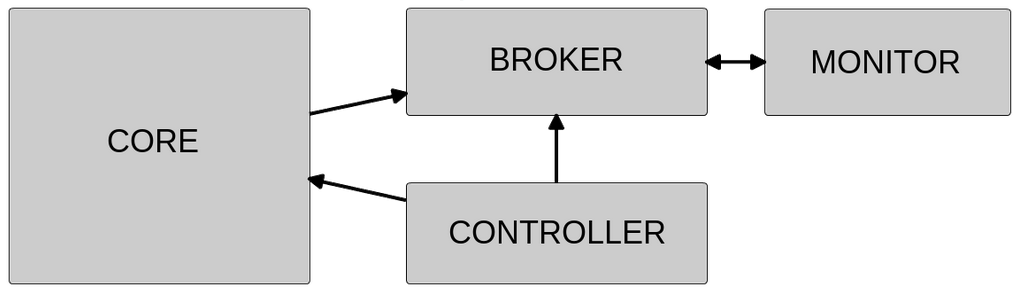
\includegraphics[keepaspectratio = true, width = 400px] {Pictures/nodes}
		\rule{35em}{0.5pt}
	\caption[Struttura]{Struttura ad alto livello.}
	\label{fig:Struttura}
\end{figure}

Come si può vedere dall’immagine, l’architettura del simulatore è stata diviso in quattro parti:
\begin{itemize}
 \item \textbf{Core}: esegue la simulazione vera e propria, calcolando i tempi, le velocità e tutto ciò che è necessario per lo svolgimento della gara
 \item \textbf{Broker}: riceve gli eventi riguardanti lo svolgimento della gara, li elabora, e li distribuisce agli elementi che ne permettono la visualizzazione ed il controllo da parte dell’utente
 \item \textbf{Monitor}: permette di visualizzare l’andamento della gara tramite una classifica ed una rappresentazione grafica dell’andamento della gara.
 \item \textbf{Controller}: dà la possibilità all’utente di agire come se fosse ai box, indicando al pilota di un veicolo che strategia utilizzare, e pianificando i pit-stop. Permette inoltre di visualizzare dati aggiuntivi sul veicolo.
\end{itemize}


Uno dei requisiti del simulatore è che sia distribuito, e quindi sorge il problema di capire quali parti possono essere separate dal core pur garantendone il funzionamento.
Ad una prima analisi del sistema abbiamo identificato quattro componenti principali per il soddisfacimento dei requisiti:
\begin{itemize}
 \item circuito
 \item macchina
 \item monitor
 \item controller
\end{itemize}
Supponiamo di dividere queste entità in nodi separati, in grado di essere eseguiti su elaboratori differenti connessi fra di loro. 
Questa partizione non funziona perchè:
\begin{itemize}
\item circuito e macchine sono funzionalmente accoppiate, l'uno necessita dell'altro per poter completare le operazioni della simulazione.
\item il distacco delle entità potrebbe causare numerosi problemi (latenza, disconnessione, ecc…) al simulatore. 
\end{itemize}
Di conseguenza è necessario che il circuito ed i veicoli siano in un unico nodo. \\

Il monitor è un’entità quasi totalmente passiva, cioè non fa altro che ricevere i dati sulla situazione della simulazione e presentarla all’utente tramite un render grafico. Dato che l’output di questa entità può essere visualizzato solo dall’utente, una possibile latenza non causa alcun disturbo, dato che può essere assimilata a ritardi causati dalla televisione in una situazione reale. Una eventuale disconnessione causata da problemi di rete potrebbe avvenire anche nel mondo reale. \\
 
Il controller è ciò che permette all’utente di decidere la strategia di gara di un dato veicolo; questo tipo di controller non necessità di avere i dati aggiornati in un tempo il più vicino possibile a quello reale, dato che non effettua un controllo diretto sul pilota ma dà solo indicazioni sulla strategia di gara, può quindi sopportare una eventuale latenza anche di qualche secondo. \\

Al termine di questa analisi i nodi identificati sono diventati tre, il core (che comprende sia il circuito che le macchine), il monitor ed il controller.
Dato che il simulatore funziona ad eventi, è sorto un ulteriore problema: il numero di eventi generati può diventare piuttosto grande, ed in caso di monitor multipli e numerosi si otterrebbe un grosso spreco di risorse inviandoli tutti (alcuni dei quali potrebbero anche non interessare al destinatario). Inoltre questi eventi andrebbero convertiti da ogni monitor in modo da poterne fare una rappresentazione, implicando inoltre un cambiamento di funzionalità del monitor, da entità passiva ad entità attiva, che raccoglie gli eventi e li elabora per creare una raffigurazione del tracciato.
Inoltre questa scelta avrebbe aumentato il carico di lavoro che grava sul core,  che avrebbe dovuto disporre di funzioni atte a permettere la comunicazione con entità multiple.
Per questi motivi abbiamo aggiunto ai tre tipi di nodi presenti un quarto, l’intermediario. Questa nuova entità (unica per tutto il simulatore) raccoglie gli eventi derivati dalla simulazione, e li elabora rendendoli facilmente fruibili per la rappresentazione grafica. In questo modo il carico di lavoro sul core viene alleggerito: dovrà comunicare gli eventi ad una sola entità. Viene anche alleggerito il carico di lavoro dei monitor, che dovranno limitarsi a fare un render grafico delle informazioni ottenute, senza essere obbligati ad avere conoscenza del funzionamento interno della simulazione.

%-----------------------------------
%	SECTION 2
%-----------------------------------
\section{Tipo di comunicazione}

Dopo aver suddiviso il simulatore in parti che possono essere distribuite su più computer, è stato necessario capire quale design pattern di comunicazione si adatti meglio al nostro utilizzo.
Le scelte analizzate sono state due:
Utilizzare un middleware
Utilizzare una libreria per lo scambio di messaggi (nel caso specifico YAMI4)
La prima permette di definire un’architettura del sistema distribuito, fissando i nodi e i ruoli di ogni agente. In questo modo si riesce a creare una distribuzione più robusta e definita a priori, che permette l’utilizzo di strutture dati interni al linguaggio in modo condiviso e trasparente.
La seconda, invece, è un insieme di librerie che espongono API che permettono l’invio di messaggi tra le varie entità del sistema distribuito; non viene definita alcuna architettura o nodo, ma viene solo fornito un sistema standard per l’invio e ricezione delle informazioni.
Per quanto la prima soluzione garantisca una maggiore affidabilità, introduce vincoli sul tipo di architettura da implementare ed una intrinseca dipendenza del software dal middleware, con la relativa necessità di installare i vari componenti prima di poter eseguire il programma.
Principalmente per questo motivo, la nostra scelta è ricaduta sulla libreria YAMI4, in quanto ci è sembrato molto importante poter garantire la portabilità di nodi quali il monitor ed il controller, in modo che possano essere avviati su pc in modalità “plug and play”, senza avere la necessità di installare ulteriore software.
Ci siamo resi conto che in una situazione diversa, ad esempio se il nostro software avesse avuto un numero di nodi molto più elevato, sarebbe stato molto rischioso affidarci ad una libreria piuttosto che ad un middleware, proprio per la caratteristica di quest’ultimo di definire ad alto livello l’intero sistema ed i vari ruoli; nel nostro caso però, la scelta di adottare una libreria per lo scambio di messaggi non ha causato problemi.

%-----------------------------------
%	SECTION 3
%-----------------------------------

\section{Comunicazione del Core}

Il core produce sequenza di eventi che indicano il raggiungimento di un obiettivo da parte di un’entità (ad esempio una macchina che esce da un segmento).
Questo flusso di eventi deve essere inviato all’intermediario, per permetterne l’elaborazione e l’invio ai monitor ed i controller.
Il tipo di comunicazione è “uno ad uno”, dato che le istanze del core e dell’intermediario sono uniche; per questo ci è sembrato appropriato utilizzare il metodo push, che invia ogni nuovo evento il prima possibile.
A differenza del pull, ogni informazione viene spedita, e la frequenza di comunicazione viene gestita dal core. Se la comunicazione fosse stata effettuata direttamente tra il core ed i monitor non sarebbe stato possibile utilizzare questo metodo, visto che ogni monitor non è interessato alla totalità di eventi. Dato che l’intermediario funziona anche come punto di raccolta delle informazioni della gara, siamo sicuri che tutti gli eventi generati dal core saranno di interesse dell’intermediario. Inoltre inviando immediatamente tutte le informazioni disponibili si diminuisce la latenza tra l’istante in cui un evento è generato e quello in cui viene ricevuto ed elaborato.
L’impegno del core dal punto di vista della comunicazione non è limitato unicamente alla trasmissione degli eventi, ma è anche necessario che sia predisposto a ricevere i comandi da parte del controller. Il ragionamento effettuato per la comunicazione core-controller è il medesimo: usando un architettura di tipo pull, sarebbe necessario che il core controllasse in continuazione se qualche giocatore ha inviato un comando, il che aumenterebbe enormemente il carico di lavoro e soprattutto avrebbe esito negativo per la maggior parte delle volte. Per questo è stato utilizzato lo stesso metodo push, ma questa volta dal controller al core (i dettagli del controller verranno descritti successivamente).

%----------------------------------------------------------------------------------------
%	SECTION 4
%----------------------------------------------------------------------------------------

\section{Comunicazione dell’intermediario}

L’intermediario deve poter comunicare su due fronti: ricevere gli eventi dal core, e inviare le informazioni elaborate al monitor ed al controller.
La comunicazione con il core è già stata trattata precedentemente: come spiegato ogni evento viene ricevuto nel modo più rapido possibile.
Dopo aver elaborato le informazioni, bisogna simistarle alle entità monitor e controller, ma la scelta del tipo di comunicazione non è banale.
Ci sono infatti diversi requisiti da soddisfare, in quanto l’intermediario è in possesso di due tipi di informazioni: quelle più generali, che servono a tutti, e quelle più dettagliate, che vengono comunicate su richiesta.
Le tipologie di invio analizzate sono principalmente due, pull e publish subscriber. Nel primo caso le informazioni devono essere recuperate esplicitamente, richiedendole all’intermediario, nel secondo ogni informazioni viene spedita a tutte le entità interessate (che hanno fatto il subscribe).
Entrambe le soluzioni hanno pro e contro, infatti utilizzare il pull implicherebbe una frequenza di aggiornamenti dettata dai monitor, e non dall’arrivo di nuove informazioni, mentre l’utilizzo del publish subscribe comporterebbe l’invio di tutte le informazioni a tutte le entità, informazioni a cui alcune entità non sono interessate, il che data la mole di informazioni sarebbe uno speco di risorse non indifferente.
Consdierato che ambedue le soluzioni hanno elementi interessanti, abbiamo deciso di utilizzarle entrambe, utilizzando una per sopperire agli svantaggi dell’altra, e viceversa.
Per questo motivo abbiamo diviso in due parti le informazioni dell’intermediario, quelle che sono necessarie a tutti, e quelle che vengono distribuite su richiesta. Per le prime abbiamo disposto un sistema di publish subscribe che le invia, appena sono disponibili, a tutte le entità registrate; per le seconde abbiamo utilizzato un sistema di pull, creando una risorsa che contiene queste informazioni, e lasciando l’onere di recuperarle all’entità interessata.

%----------------------------------------------------------------------------------------
%	SECTION 5
%----------------------------------------------------------------------------------------

\section{Comunicazione del monitor}

Come detto precedentemente il monitor deve ricevere i dati elaborati dall’intermediario per poter effettuare la rappresentazione grafica.
Tuttavia sono necessari dati aggiuntivi a quelli dell’andamento della gara per poter fare una buona rappresentazione, come ad esempio il numero di partecipanti e di giri, che data la loro staticità durante l’evoluzione non hanno motivo di essere inviati ad ogni publish. Per questo motivo prima di registrarsi alle pubblicazioni dell’intermediario, il monitor recupera in pull queste informazioni aggiuntive tramite la richiesta di un setup.
Completato questo passo la comunicazione continuerà in publish subscribe fino alla fine della gara.

%----------------------------------------------------------------------------------------
%	SECTION 6
%----------------------------------------------------------------------------------------

\section{Comunicazione del Controller}

Il controller permette all’utente di ottenere informazioni aggiuntive riguardo uno specifico veicolo, e offre la possibilità di modificarne le strategie.
La comunicazione si divide quindi in due parti, ricezione dei dati, ed invio.
Riguardo la ricezione viene utilizzato il metodo descritto sopra, e dato che questi dati sono aggiuntivi rispetto a quelli della gara verranno reperiti tramite pull dall’intermediario.
Per l’invio invece, l’idea iniziale è stata quella di inviare le informazioni all’intermediario che si sarebbe poi  occupato di farle arrivare al core. Il problema di questo approccio è dato dal tipo di informazioni che inviamo, infatti a differenza di una semplice visualizzazione grafica che può sopportare una latenza anche di qualche secondo, i dati riguardanti la strategia possono cambiare il corso della gara, ed è quindi necessario farli arrivare al core il prima possibile. Per questo ogni comando dell’utente viene spedito tramite un canale a parte che va dal controller al core, utilizzando il metodo push. In questo modo il core dovrà solo rimanere in ascolto, senza alcun carico di lavoro supplementare. 
Un ulteriore problema può essere causato dal fatto che ciò che vede l’utente dal monitor non è perfettamente in tempo reale, ma soffre di una leggera latenza causata dalla rete e da tutti i calcoli dell’interpolazione dei dati per il rendering grafico. Considerato che i comandi dati dall’utente riguardano esclusivamente la strategia, e non il comportamento immediato del veicolo, siamo giunti alla conclusione che questo non causa un problema nello specifico. Le informazioni sulla strategia infatti non hanno un esecuzione immediata, e quindi possono tranquillamente sopportare una breve latenza.

%----------------------------------------------------------------------------------------
%	SECTION 7
%----------------------------------------------------------------------------------------

\section{Avvio e chiusura del sistema}

Un grosso problema di un sistema distribuito è quello di organizzare l’avvio e la chiusura dell’intero sistema.
Il core e l’intermediario hanno funzioni fortemente correlate, quindi non è stato nemmeno presa in considerazione l’eventualità in cui l’intermediario si possa connettere a gara iniziata
Le situazioni possibili sono due: se durante il bootstrap la comunicazione tra i due va a buon fine, il core lavorerà in modalità distribuita inviando tutti gli eventi all’intermediario man mano che vengono generati; in caso contrario il core eseguirà in modalità locale, consumando gli eventi con delle stampe a schermo degli avvenimenti della gara. Quest’ultima modalità di esecuzione non genera contenuti fruibili per un utente, ed è quindi stata creata solo per motivi di debug.
Quando l’intermediario viene avviato, attende come primo messaggio una comunicazione da parte del core contenente la configurazione della gara. Una volta ricevuto quel messaggio, disporrà le risorse necessarie per permette la comunicazione con il controller ed il monitor.
Questi ultimi due componenti sono stati progettati con l’intento di renderli collegabili e scollegabili a piacere, e possono essere avviati anche a gara iniziata. Questo può essere associato alla realtà con l’idea di poter accendere e spegnerein qualunque momento la TV con cui si guarda la gara o la radio con cui si comunica ai piloti.
Ottenere una chiusura ordinata, invece, ha richiesto l’uso di elementi aggiuntivi. Ogni entità è stata progettata per arrestarsi automaticamente al segnale di chiusura, non forzando l’utente a dover utilizzare CTRL-C o altri comandi di chiusura forzata per terminare l’applicazione.
Quando anche l’ultimo veicolo è arrivato al termine della gara, il core invita ogni task alla chiusura; prima di concludere le attività viene però inviato un evento speciale che indica la conclusione della gara, come ogni evento anche quest’ultimo verrà ricevuto dall’intermediario (per come è stato costruito) che sarà quindi informato del fatto che la gara è terminata. Come per il core, anche l’intermediario comunicherà a tutti i task di cui è composto che la chiusura è imminente.
Il caso del monitor e del controller è leggermente diverso, infatti mentre è auspicabile la chiusura del terminale per il core e l’intermediario, la chiusura improvvisa della finestra di visualizzazione potrebbe non essere altrettanto piacevole per l’utente. In questo caso la terminazione delle altre entità non causerà la chiusura, ma solo una comunicazione all’utente della nuova situazione. A questo punto sarà onere dell’utente chiudere la finestra quando lo riterrà più opportuno, e solo allora il monitor ed il controller si chiuderanno. 
% Chapter Template

\chapter{Soluzione proposta} % Main chapter title

\label{Chapter6} % Change X to a consecutive number; for referencing this chapter elsewhere, use \ref{ChapterX}

\lhead{Capitolo 6. \emph{Soluzione proposta}} % Change X to a consecutive number; this is for the header on each page - perhaps a shortened title

%----------------------------------------------------------------------------------------
%	SECTION 1
%----------------------------------------------------------------------------------------

\section{Linguaggi}

Per l’implementazione del progetto sono stati utilizzati due linguaggi. Per tutta la parte con requisiti di mutua esclusione, accodamento e multithreading è stato utilizzato Ada, data la sua predisposizione di primitive a supporto della gestione dei thread e delle risorse protette, che hanno reso lo sviluppo più facile ed affidabile. Ad esempio l’implementazione delle risorse protette, la relativa mutua esclusione e l’accodamento sarebbe stata molto più complessa (e a rischio di errore) utilizzando un altro linguaggio. \\
Tutta la parte grafica (monitor e controller) non ha requisiti di concorrenza tra più thread, e per questo è stato utilizzato Java e le sue librerie grafiche (swing e awt). Questa scelta è stata dettata dalla facilità implementativa che Java offre nel reparto grafico, e anche dal desiderio di utilizzare l’occasione per imparare una delle librerie più utilizzate per la costruzione di GUI. Inoltre Java offre una portabilità maggiore, e associato a YAMI4 (anch’esso portabile) è sembrato un valore aggiunto dare la possibilità di portare il monitor ed il controller su altri PC senza la necessità di ricompilare, dato che sono le due entità che si prestano meglio ad essere usate in modalità “plug and play”.
\newpage
%----------------------------------------------------------------------------------------
%	SECTION 2
%----------------------------------------------------------------------------------------

\section{Componenti ad alto livello}

\begin{figure}[htbp]
	\centering
		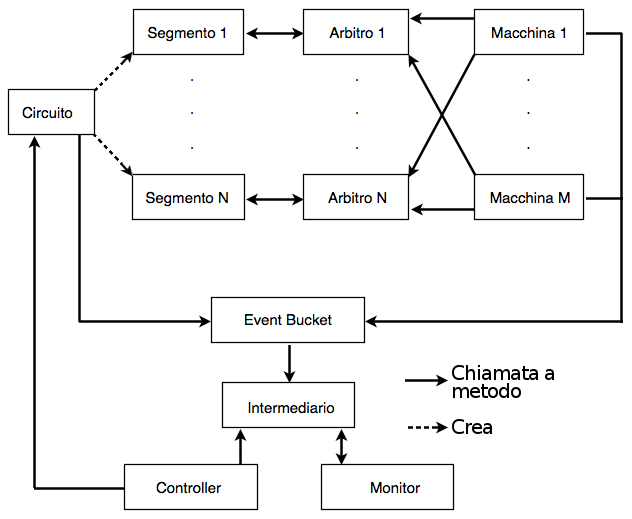
\includegraphics[keepaspectratio = true, width = 380px] {Pictures/schema}
		\rule{35em}{0.5pt}
	\caption[Componenti]{Componenti: visione ad alto livello delle componenti del sistema.}
	\label{fig:Componenti}
\end{figure}

\subsection{Circuito}

Come detto precedentemente il circuito viene rappresentato come una sequenza di segmenti. Ognuno di questi contiene le caratteristiche necessarie a descrivere il tratto associato: la lunghezza in metri, la molteplicità, ed un grado di difficoltà (da 1 a 10) che permette di discriminare le tipologie dei tratti (un rettilineo ha una difficoltà di 1, le curve variano da 2 a 10, a seconda dell’angolo descritto). Inoltre è stata aggiunta una variabile booleana per indicare se nel tratto è presente l’ingresso ai box.
All’interno del circuito è anche presente una entità attiva, che rappresenta il meteo. Questo task genera cambi casuali di tempo atmosferico, rendendo più realistica la gara, e generandone gli eventi relativi.
I dati relativi al tracciato vengono letti da un file “circuit.txt”, tramite un parser implementato ad hoc che processa le informazioni contenute nel file per costruire una struttura dati interna che si occupa di memorizzare tutte le informazioni necessarie.

\subsection{Arbitro}

L’arbitro è l’entità passiva che si interpone tra i veicoli ed un certo segmento. La sua utilità è molteplice, permette infatti di calcolare il tempo di attraversamento di un tratto dati i parametri della macchina, ed evita il formarsi di code di task in attesa per l’ingresso in un segmento fornendo subito una risposta. Possiamo dire che il vero lavoro di calcolo fisico della simulazione viene effettuato dall’arbitro, togliendo la possibilità alle macchine di autodeterminarsi.
I canali principali di questa entità sono due: la procedure “enterSegment” e “leaveSegment”, entrambe utilizzate dai task dei veicoli.
La prima viene chiamata quando una macchina richiede l’ingresso al segmento successivo a quello in cui si trova, e si affida all’arbitro per verificare la situazione ed agire di conseguenza.
Le possibilità sono due: se il numero di veicoli già presenti nel tratto è minore della molteplicità del medesimo (ad esempio se è vuoto), l’arbitro utilizzerà semplicemente i parametri del veicolo per calcolare la nuova velocità di uscita ed il tempo impiegato; in caso contrario, l’arbitro è obbligato a considerare il segmento saturo, e per questo dovrà sommare al tempo che la macchina avrebbe impiegato ad attraversare il tratto,  quello necessario a liberare il medesimo da un numero di veicoli sufficienti in modo che non possa più essere considerato saturo. Considerato che il tempo di uscita viene calcolato proprio dall’arbitro, è facile tenerne traccia per essere sempre a conoscenza di quando il tratto avrà posto disponibile. Anche nel secondo caso al termine del calcolo vengono restituiti alla macchina il tempo di attesa e la nuova velocità. Quest’ultima in questo caso sarà ridotta in modo da rispecchiare la decelerazione causata dalla presenza di una macchina che al momento non è superabile (data la saturazione della molteplicità).
In entrambi i casi la macchina è ignara dell’accaduto, nel senso che non sarà obbligata a restare in attesa su code o eseguire lavoro aggiuntivo. \\
Il secondo canale dell’entità arbitro, il “leaveSegment”, viene usato (come suggerito dal nome) per liberare il segmento da una macchina che ne è uscita. Dato che l’arbitro è a conoscenza dell’istante di uscita ogni veicolo, una scelta possibile sarebbe stata quella di non disporre questo secondo canale, e gestire tutto internamente all’arbitro. Il problema di questa scelta è dato dal fatto che quest’ultimo è un’entità passiva, ed è per questo impossibilitata ad effettuare controlli o ad intraprendere azioni attivamente. Inoltre dato che è la macchina l’entità attiva, è sembrato sensato far compiere a lei le due azioni che implicano l’avanzamento della gara, cioè l’ingresso e l’uscita dal segmento. L’unico inconveniente che potrebbe sorgere è un possibile incremento ingiustificato del tempo di permanenza all'interno del segmento, causato dal fatto che “leaveSegment” è una procedure di una risorsa protetta, e quindi è in mutua esclusione con la procedure “enterSegment”; il problema è stato risolto imponendo by design che due o più veicoli non si risveglino contemporaneamente, ma sia sempre presente uno scarto temporale. L'algoritmo specifico verrà trattato successivamente.
Inoltre l’unica azione che viene compiuta dalla “leaveSegment” è quella di decrementare un contatore interno relativo al numero di macchine presenti nel segmento, che essendo una semplice operazione aritmetica viene eseguita senza sideeffects.


\subsection{Car}

Ogni vettura che partecipa alla gara è un’entità attiva separata, dotata di parametri propri che cercano di rispecchiare le caratteristiche di un veicolo reale. Questi parametri vengono letti all’avvio del core, da un file “cars.txt” tramite parser. Dopo la lettura i task vengono creati utilizzando le informazioni lette dal file. Tra i parametri figurano velocità massima in $Km/h$, l’accelerazione in $m/s^2$, il comportamento del pilota (che implica la strategia), ed il suo identificativo. Inoltre sono presenti numerose altre informazioni che raffigurano lo stato in gara, come lo stato ed il tipo di gomme, i danni riportati in caso di incidente e la velocità istantanea.
Il ciclo di vita dei task macchina è relativamente semplice, infatti consiste nel richiedere l’ingresso in un segmento, attendere quanto specificato dall’arbitro, ed uscire dal segmento.
Questo ciclo viene ripetuto finchè i giri non terminano, o fino al ritiro del veicolo in caso di incidente.
L’attesa tra l’ingresso in un segmento e l’uscita dal medesimo viene fatta tramite il costrutto “delay until”, che ci assicura che in caso il risveglio del task ottenga qualche ritardo, quest’ultimo non venga accumulato al risveglio successivo.
Inoltre la macchina ha l’onere di generare gli eventi che la riguardano, come ad esempio l’uscita da un segmento o il verificarsi di un incidente.

\subsection{Raccoglitore di eventi}

Data la grande mole di eventi generati durante la gara, sarebbe stato poco funzionale farli inviare all’intermediario direttamente dall’entità che li genera. Il rischio che si sarebbe corso è quello di far perdere tempo ad un entità attiva, che è un comportamento poco desiderabile. Per questo è stato deciso di slegare completamente la creazione di un evento dalla sua distribuzione. Per farlo viene creato un raccoglitore di eventi, o event bucket, che funziona con il classico paradigma produttore-consumatore; infatti ogni entità che produce eventi si occupa di inserirli in questo “secchio”, e sarà poi onere di qualcun altro consumarli adeguatamente.
Questa nuova figura è un’entità attiva che raccoglie gli eventi depositati e li invia all’intermediario tramite l’interfaccia di invio messaggi di YAMI4. Per evitare il busy-waiting è stato disposto un canale con guardia nel raccoglitore di eventi, in modo che il task di invio resti in attesa nell’entry finché la guardia non si apre (indicando la presenza di nuovi eventi da consumare) e li invia.
Scollegando la produzione dal consumo ci siamo assicurati che il funzionamento del sistema non sia dipendente da problemi esterni, come ad esempio malfunzionamenti della rete.

\subsection{Intermediario}

Il compito dell’intermediario è duplice, infatti oltre a dover comunicare con tutti gli altri nodi del sistema, ha anche il compito di elaborare gli eventi ricevuti dal core per renderli fruibili dall’utente attraverso il monitor.
In questo caso il problema da considerare non è banale, infatti ciò che viene ricevuto dal core è una sequenza di eventi, scanditi dal raggiungimento di alcuni obiettivi della gara (ovvero tempo in funzione dello spazio). Ciò che invece sarebbe auspicabile visualizzare per l’utente, è una sequenza continua che indica in ogni istante la situazione della gara, ovvero spazio in funzione del tempo. Quindi è necessario passare da informazioni basate sullo spazio (come una macchina che esce da un segmento) ad una rappresentazione temporale (uno snapshot di tutti i veicoli in un certo istante) come quello che si può vedere in TV durante le gare di F1.
L’intermediario ha quindi l’obbligo di interpolare i dati a disposizione per ricreare la situazione di gara, utilizzando i dati a disposizione (velocità, tempi di uscita, ecc…) per approssimare la posizione di ogni veicolo anche quando non ci sono informazioni disponibili (ad esempio quando la macchina è in attesa di uscire da un tratto).
Per questo vengono creati degli snapshot con una frequenza di mezzo secondo l’uno dall’altro, in cui sono contenute tutte le posizioni dei veicoli e la relativa situazione nella classifica; queste informazioni vengono inviate appena possibile ai monitor.
La creazione dello snapshot introduce anche un problema, infatti per rendere l’istantanea più corretta possibile, viene introdotta una breve latenza, in modo da permettere agli eventi attesi un piccolo margine di tempo per arrivare. Dato che gli eventi vengono salvati in alcune liste circolari, ed il tempo di esecuzione è relativo (ogni tempo si riferisce sempre all’istante zero) è stato introdotto un ritardo artificiale tra il tempo reale e quello dell’ultimo snapshot, creando un piccolo buffer logico che aumenta di molto la precisione delle previsioni effettuate. Tuttavia questo implica che il monitor visualizzerà la gara con ritardo di 1-2 secondi. Questa soluzione resta preferibile poichè la latenza è costante, e può essere associata al problema reale del ritardo che intercorre tra l’invio delle immagini e la relativa ricezione e visualizzazione nella TV. Anche nel controller la cosa non ha un impatto problematico, infatti come detto precedentemente tutti i comandi che l’utente può comunicare non sono pensati per agire in tempo reale, ma essendo strategie posso soffrire di una breve latenza senza inficiarne le funzionalità.

\subsection{Monitor}

Il monitor ha la funzione di permettere all’utente di seguire graficamente lo svolgimento della gara. Come spiegato nel precedente paragrafo, tutte le informazioni vengono comunicate tramite snapshot al monitor, che le elabora costruendo una interfaccia di facile comprensione per l’utente.
La finestra che viene presentata è pensata per contenere i dati comuni a cui ogni utente è interessato, ed è quindi contenuta la rappresentazione grafica della gara e la classifica dinamica che riflette la situazione corrente dei partecipanti, comprensiva di distanza temporale dal primo classificato. In quest’ultimo elemento vengono anche incluse le informazioni più rilevanti relative ad ogni veicolo, come l’ingresso ai box o il verificarsi di incidenti.
Tutte le informazioni aggiuntive possono essere reperite dal controller.

\subsection{Controller}

Il controller permette di visualizzare informazioni aggiuntive su un certo veicolo, e dà la possibilità all’utente di modificare il comportamento del pilota (strategia) e di organizzare i rientri ai box. 
In linea teorica i dati ricavati dal controller non hanno bisogno di elaborazione, e quindi a differenza del monitor non soffrono della latenza necessaria alla creazione dello snapshot.
A questo punto è però sorto un problema, infatti il controller ed il monitor sono stati concepiti per essere utilizzati assieme, e non come elementi separati.  Senza pre-elaborazione dei dati aggiuntivi  nelle due finestre sarebbero stati presenti dati provenienti da due istanti leggermente diversi. Per rendere l’esperienza migliore, e considerato che la latenza è fissa e nota a priori, è stato deciso di aggiungere ai dati del controller lo stesso ritardo da cui sono affetti gli snapshot, in modo che le informazioni ottenute dalle due finestre siano perfettamente sincronizzate.

\section{Implementazione nel dettaglio}

Verrà ora descritta l’implementazione in modo dettagliato, per ogni package$/$classe più importante.
\begin{figure}[htbp]
	\centering
		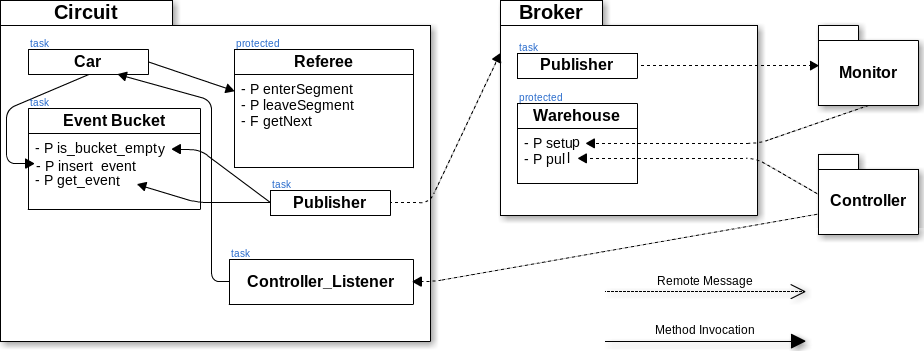
\includegraphics[keepaspectratio = true, width = 400px] {Pictures/SchemaOverview}
		\rule{35em}{0.5pt}
	\caption[Componenti]{Componenti: vista in dettaglio.}
	\label{fig:SchemaOverview}
\end{figure}

\subsection{Circuit}

Il package Circuit ha il compito di inizializzare tutte le componenti della simulazione. 
Il suo task bootstrap è responsabile di avviare la creazione della pista, attraverso un parser che legge le informazioni dei segmenti da un file di testo “circuit.txt”. Nel file di rappresentazione della pista sono presenti tante righe quanti sono i segmenti del tracciato, e ogni riga contiene cinque dati: l’identificatore del segmento, la lunghezza, la molteplicità, la difficoltà, e una variabile booleana che indica l’eventuale ingresso ai box.
Come spiegato precedentemente, le vere risorse protette sono rappresentate dall’arbitro, mentre i segmenti generati finora sono le descrizioni dei vari tratti. Sempre nell’inizializzazione, quindi, vengono creati gli arbitri, e ad ognuno viene assegnato il relativo tratto di competenza.
Un procedimento analogo viene fatto per le caratteristiche dei veicoli, che vengono anch’esse lette da un file di testo cars.txt”, in cui ogni riga indica i parametri di una macchina; sono presenti quattro valori, l’id, il comportamento di default, la velocità massima, e l’accelerazione.
Per ogni riga viene creato un oggetto ``car\textunderscore status'' che verrà poi passato al task ``car\textunderscore p'' creato di conseguenza, che lo userà per leggere e salvare lo stato del veicolo rappresentato.
Le ultime cose che vengono effettuate nel bootstrap è l’inizializzazione e l’avvio del task “controller”, che predispone l’ascolto per l’override sul comportamento da parte dell’utente, ed il task publisher, che si occupa di inviare all’intermediario tutti i nuovi eventi.
Appena i task delle macchine vengono creati vengono messi in stato di sleep. Il tempo di risveglio è diverso fra le varie auto in modo da evitare l'accesso contemporaneo alla procedure del primo segmento. Senza di un controllo ogni macchina sarebbe partita appena creata, creando un vantaggio non controllabile dettato dallo scheduler per i primi veicoli inizializzati; in questo modo invece, le prime macchine create hanno un tempo di risveglio minore delle successive, creando una linea di partenza virtuale (basata sull’ordine dei veicoli indicati sul file di configurazione). Utilizzando questa soluzione il realismo della partenza viene rispettato, ed è implementato in modo che i task delle macchine non dovranno autonomamente controllare un flag ma saranno automaticamente svegliate dalla macchina astratta appena sarà il loro turno.
Dopo aver avviato la gara il task bootstrap si conclude. \\
Il Circuit contiene anche il task del meteo, che tramite la generazione di un numero casuale calcola un tempo di attesa prima del cambio di condizioni metereologiche. Per rendere più realistica questa componente, il tempo di attesa potrebbe essere anche più lungo del tempo totale di gara, implicando il mantenimento dello stesso stato per tutta la durata della competizione. Nell’attesa il thread è in stato di sleep, anche se viene risvegliato ogni 5 secondi per controllare se la gara è ancora in corso; questa condizione è stata resa necessaria per permettere la chiusura ordinata del programma, infatti è obbligatorio che il task controlli periodicamente se la competizione è terminata, chiudendosi assieme agli altri task in caso affermativo. Se non risvegliassimo il task del meteo ogni 5 secondi, ma ci limitassimo a svegliarlo solo quando deve cambiare stato, prima della chiusura del core dovremmo aspettare un tempo molto lungo e quindi proibitivo.

\subsection{Referee}

Come ampiamente anticipato, il referee (o arbitro) è l’entità che incarna la vera risorsa protetta del segmento. 
Oltre al alcune funzioni e procedure necessarie per il setup, i canali principali che offre sono tre, “getNext”, “enterSegment”, “leaveSegment”.
La prima è una funzione rispecchia l’implementazione a linked list, in cui ogni elemento conosce solo i propri dati ed un puntatore all’elemento successivo.
La maggior parte del lavoro viene effettuata dalla procedure “enterSegment”, che ha l’onere di calcolare tramite vincoli fisici l’attraversamento del segmento da parte del veicolo o il suo ingresso ai box.
Per ricavare il tempo di attesa e la nuova velocità vengono utilizzate le leggi della cinematica modificate con coefficienti che alterano il risultato a seconda della strategia utilizzata dal pilota e dal tipo di tratto. Per quanto nella realtà l’accelerazione non sia costante, ci è sembrata una buona approssimazione, soprattutto considerando che il realismo fisico non è il fine ultimo del progetto.

\noindent%
\begin{minipage}{\linewidth}
\makebox[\linewidth]{%
  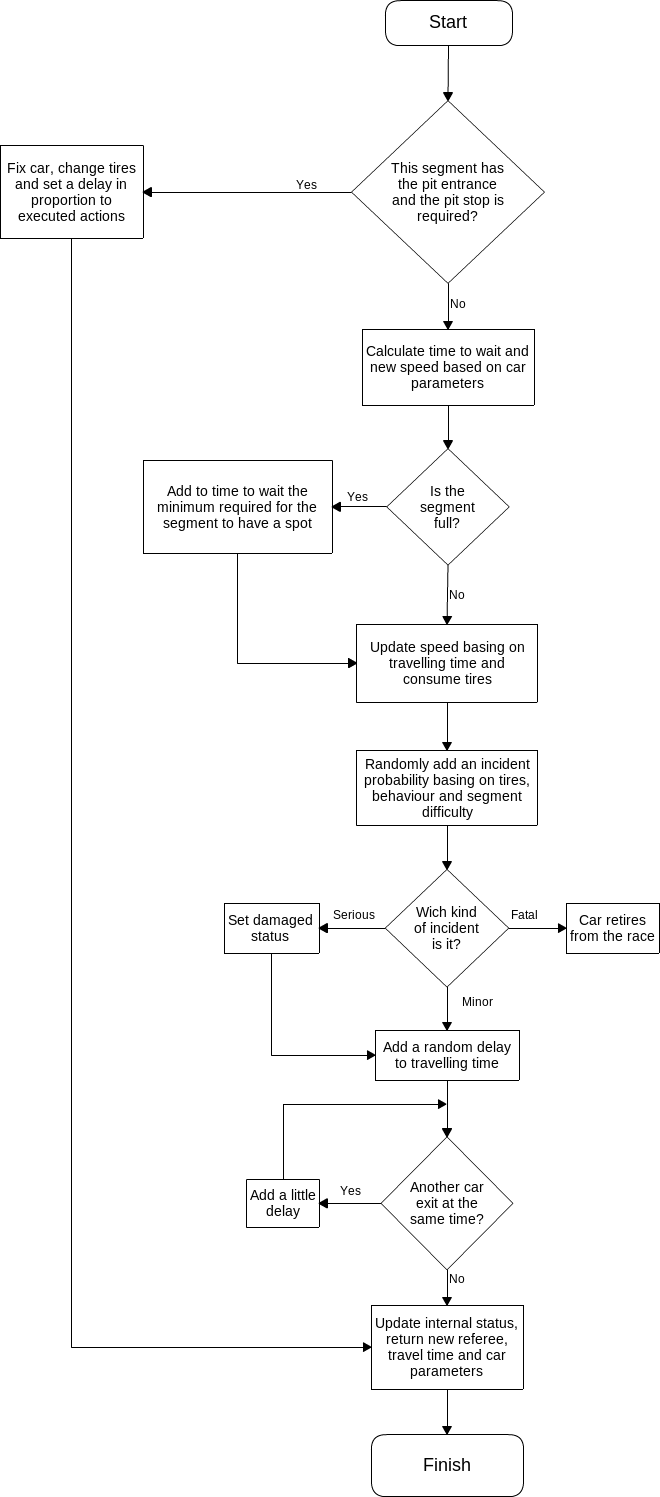
\includegraphics[keepaspectratio=true,scale=0.4]{Pictures/enterSegment}}
\captionof{figure}{Flowchart: procedure enterSegment.}% only if needed
\label{enterSegment}
\end{minipage}

Dopo aver calcolato il tempo di attesa e la nuova velocità del veicolo, viene effettuato un controllo sulla molteplicità del tratto, verificando il numero di veicoli al momento presenti all’interno. In caso ci sia spazio per un’altra macchina, il tempo e la velocità restano invariate, dato che rappresentano il massimo che la vettura può ottenere; in caso contrario la vettura deve accodarsi alla più vicina che la precede, e viene quindi sommato al tempo di uscita del veicolo il minor tempo per permettere l’uscita di una delle macchine già presenti.
Essendo in possesso del nuovo tempo di uscita viene ricalcolata la velocità, simulando la frenata necessaria ad adeguarsi al veicolo che la precede.
L’arbitro provvede anche ad aggiornare lo stato delle gomme dei veicoli, calcolandone il consumo basato sul tratto percorso, sul comportamento del pilota, ed in piccola parte dalla casualità (che aggiunge una piccola parte di non determinismo). La variabile che rappresenta lo stato attuale delle gomme viene utilizzata per eseguire il rientro ai box per il cambio gomme quando quest’ultime sono troppo usurate.
Successivamente viene calcolata la probabilità di incidente, che si basa su un calcolo che utilizza sia elementi casuali che coefficienti riguardanti lo stato della pista, il comportamento del pilota, il meteo, e l’adeguatezza delle gomme alla situazione atmosferica. La probabilità di incidente in uscita dal segmento varia dallo 0.1\% in condizioni favorevoli, allo 0.4\% in condizioni difficili.
In caso di uscita è presente un 10\% di probabilità di danneggiamento del veicolo, e un 5\% di probabilità di rottura irrimediabile che causi il ritiro.
Il referee ha inoltre il dovere di gestire l’ingresso ai box nel caso sia proprietario di un tratto con ingresso al pit stop. I box non sono rappresentati da un vero segmento, ma sono invece espressi da uno stato logico; quando l’arbitro deve far entrare un veicolo ai box agisce diversamente, calcolando un tempo di uscita basato sulla necessità di riparazioni o il semplice cambio gomme. È stato scelto di non creare una tipologia diversa di segmento per la gestione del box perché dato che l’output resta sempre il tempo di attesa e la velocità di uscita, sarebbe stato creato qualcosa di nuovo per gestire una azione che viene già supportata dal referee. La soluzione adottata è quindi di far calcolare il tempo di uscita in base alle azioni intraprese nei box (cambio gomme/riparazioni) e restituire alla macchina il segmento di uscita dai box invece che quello successivo. Quando alla macchina sarà comunicato il nuovo stato genererà un evento relativo ai box invece che quello relativo ad un semplice segmento.

\subsection{Car}

Il task Car, contenuto nel package car\textunderscore p, è ciò che rappresenta il funzionamento di una macchina che partecipa alla competizione.
Il suo ciclo di vita consiste in due azioni principali, la richiesta di ingresso in un segmento, e l’applicazione delle istruzioni restituite dal referee.

\noindent%
\begin{minipage}{\linewidth}
\makebox[\linewidth]{%
  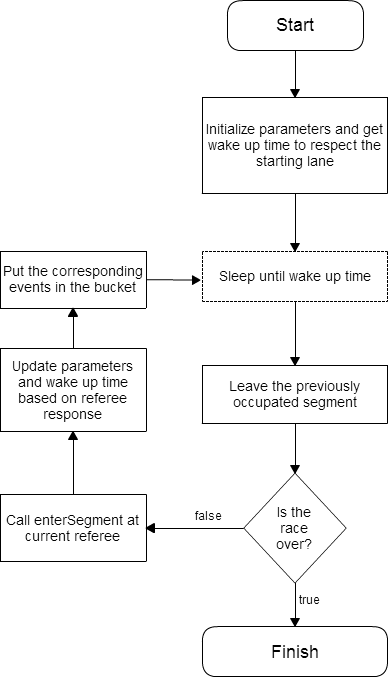
\includegraphics[keepaspectratio=true,scale=0.5]{Pictures/car_p_ciclo}}
\captionof{figure}{Flowchart: ciclo di vita di car.}% only if needed
\label{car_p_ciclo}
\end{minipage}

Per la prima, viene utilizzata la procedure “enterSegment” del referee, a cui vengono passati i parametri attuali, e si aspetta in uscita i dati neccessari a proseguire, cioè il tempo di attesa, un puntatore al prossimo arbitro da contattare, ed il nuovo stato del veicolo.
A questo punto il task deve controllare i dati restituiti, ed agire di conseguenza. I casi possono essere molteplici, e per questo deve generare gli eventi necessari per spiegare l’andamento di una gara, comunicando un eventuale incidente (con possibili danni o ritiro), il rientro ai box, o la semplice uscita del segmento (associata alla nuova velocità, strategia e gli altri dati necessari all’intermediario).
Il tempo di attesa è stato implementato con un “delay until”, che a differenza del semplice “delay” permette di ottenere una precisione migliore e non causa latenza incrementale. Per questo è stato necessario avere un riferimento assoluto di tempo. La scelta è stata quella di leggere il clock del PC solo una volta, all’avvio del task, e sommare di volta in volta il tempo di attesa derivante dall’attraversamento del segmento.
In questo modo anche se la macchina dovesse impegare del tempo per inviare gli eventi al raccoglitore, o se venisse svegliata più tardi di quanto richiesto, non accumulerebbe alcuna latenza, dato che il momento del risveglio è già stato fissato, ed il tempo di elaborazione è molto più piccolo di quello di attesa.

Per dimostrarlo è stato calcolato in modo empirico il tempo di esecuzione della chiamata a procedure enterSegment. Per eseguire il test è stato inserito un solo veicolo e sono stati rilevati i tempi assoluti del sistema prima e dopo la chiamata a procedure. Il caso peggiore rilevato ha evidenziato un periodo di $32 \cdot 10^{-6}$ secondi, approssimato per eccesso a $50 \cdot 10^{-6}$ secondi. Considerando che il numero massimo di vetture in esecuzione concorrente è di 20, possiamo fissare il tempo massimo di attesa a $20 \cdot 50 \cdot 10^{-6}$ s, cioè 1 ms. Per questo motivo l'$\mathcal{E}$ discusso in \ref{epsilondeterminismo} è stato fissato a questo valore.

Un’altra scelta possibile sarebbe stata quella di far inviare gli eventi direttamente dall’arbitro, ma aggiungere del lavoro all’interno di una risorsa protetta è una cattiva idea in quanto può tranquillamente occuparsene un task durante le attese.
Al risveglio la macchina provvede ad avvisare l’arbitro della sua uscita dal segmento, e continua il ciclo finchè non terminano i giri, o un incidente la costringe al ritiro. In entrambi i casi, prima di concludere il task, la vettura comunica all’entità che mantiene lo stato della gara la sua uscita dalla competizione, in modo che quando non ci sarà più nessun veicolo in corsa potrà comunicare la fine della simulazione e chiudere in modo ordinato.
Oltre alla comunicazione degli eventi la macchina si occupa anche di compiere alcune operazioni di default, come programmare il rientro ai box per il cambio gomme in caso di pioggia o di usura, o in caso di danneggiamento di conseguenza ad un incidente. La sosta ai box può anche essere programmata dall’utente, facendo override sul comportamento di default della macchina.
%TODO sono arrivato fino a qui, 28//11/13 12.38
\subsection{Event Bucket}

L’event bucket è una risorsa protetta presente all’interno del package event\textunderscore bkt. Il suo scopo è quello di raccogliere gli eventi provenienti dalle varie entità del core, e renderle disponibili ad un task che le invii all’intermediario.
Come già anticipato, la sua funzione è quella di “magazzino”, in cui i produttori mettono gli eventi in attesa che il consumatore li raccolga, ed è stato implementato per permettere la separazione logica tra chi produce e chi consuma, non obbligando il contatto diretto (che comporta possibili perdite di tempo).
All’inizializzazione viene definita la sua capacità, che deve essere abbastanza ampia per gestire la raccolta di eventi in rapida successione.
Le funzioni principali si raggiungono con tre canali, “insert\textunderscore event”, “get\textunderscore event” e “is\textunderscore bucket\textunderscore empty”.
La procedura “insert\textunderscore event” viene chiamata da tutti i produttori, e serve ad inserire l’evento all’interno del bucket. Ogni evento è rappresentato da un array di stringhe, contenente i vari dati relativi. Il bucket invece, è stato implementato come un vector, data la sua predisposizione ad essere gestito come una coda FIFO. All’inserimento di ogni evento un contatore aumenta, tenendo sempre conto del numero di elementi non ancora consumati.
L’entry “get\textunderscore event” restituisce il primo elemento della coda, e diminuisce il contatore degli eventi. All’ingresso di questa entry è stata posta una guardia, che si apre solo quando è presente almeno un elemento.
La procedura “is\textunderscore bucket\textunderscore empty” restituisce un valore booleano che indica se il bucket è vuoto; la sua necessità risulta evidente nel momento di chiusura dei task a termine della gara, infatti se il task di invio terminasse solo perché ogni veicolo ha raggiunto il termine, potrebbe non inviare gli ultimi eventi in coda, e per questo la terminazione è basata anche sulla quantità di eventi rimanenti.

\subsection{Publisher}

Il publisher si occupa di “impacchettare” i messaggi ed inviarli al broker. Come detto precedentemente, i messaggi vengono salvati nel broker come array di stringhe, mentre il messaggio che verrà inviato è implementato come una lista di coppie chiave/valore.
Ogni evento è identificato dall’attributo type, che può essere di otto tipi:

\begin{itemize}
 \item Eventi generati dai veicoli
 \begin{itemize}
  \item ES indica l’uscita da un segmento
  \item EB indica l’ingresso ai box
  \item LB indica l’uscita dai box
  \item EL indica la fine di un giro
  \item CE indica la fine della gara
  \item CA indica un incidente
 \end{itemize}
 \item ER indica la fine della gara
 \item SE indica il setup
\end{itemize}

Il primo compito è quello di recuperare gli eventi dal bucket, e convertirli da array di stringhe a liste di coppie. Ogni tipo di evento ha un numero fissato di parametri da contenere, quindi durante la conversione deve esclusivamente controllare la tipologia di evento per sapere come procedere.
Una volta creato l’evento viene inviato immediatamente al broker.

\subsection{Broker}

Il broker, o intermediario, si occupa di mediare la comunicazione fra il core principale che esegue la simulazione, e gli eventuali monitor o controller che vogliono visualizzarne lo stato in un dato istante. Ottiene il duplice scopo di bilanciare il traffico di rete e di processare i dati forniti dal simulatore in modo che siano più facilmente fruibili per la visualizzazione. Infatti, ponendosi a metà tra monitor e core, permette di alleggerire il carico di lavoro del simulatore poichè la comunicazione di quest’ultimo sarà sempre solo con un entità singola (il broker), indipendentemente dal numero di monitor che stanno visualizzando la gara in un dato istante.
Come prima cosa apre un canale di comunicazione che il core utilizzerà per inviare gli eventi man mano che vengono prodotti, tramite un architettura push. Gli eventi vengono smistati in base al loro tipo, e memorizzati nello stato interno del broker utilizzando una lista circolare. In questo modo riusciamo a mantenerne uno storico. L’utilizzo di una lista circolare è stato dettato dal fatto che per ragioni di memoria limitata non possiamo memorizzarli tutti. In questo modo quando lo spazio è esaurito gli eventi più recenti vengono sempre memorizzati, ricavando spazio dalla rimozione di quelli più obsoleti.
Gli eventi così memorizzati vengono poi elaborati in modo da ricavare uno snapshot, ovvero una “fotografia” della gara in un dato istante, fruibile dal monitor per la visualizzazione. Questo è necessario perchè gli eventi generati dal core si riferiscono al dominio dello spazio, ma per poter essere fruibili da un utente umano è necessario che essi siano nel dominio del tempo.
La costruzione dello snapshot viene effettuata ripetutamente a intervalli discreti e regolari.
Gli eventi ricevuti dal monitor contengono tutti un timestamp, ovvero il tempo in millisecondi relativo dall’inizio della simulazione in cui sono stati generati. La maggior parte di essi contiene anche il numero identificativo della macchina che li ha prodotti. Grazie a questi due campi è possibile raggruppare eventi che si riferiscono alla stessa macchina, e ordinarli in base al timestamp in modo crescente.

\noindent%
\begin{minipage}{\linewidth}
\makebox[\linewidth]{%
  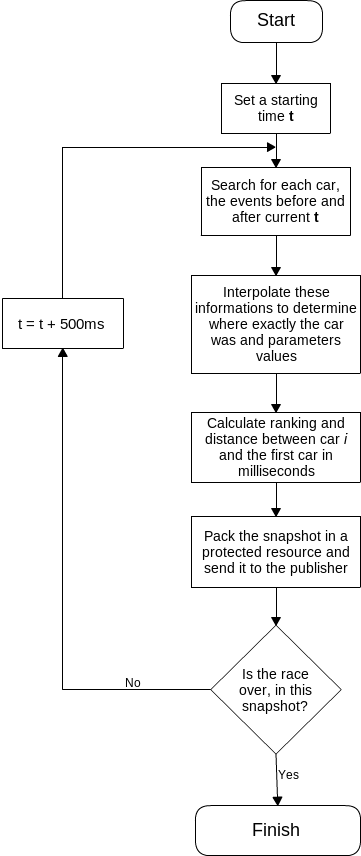
\includegraphics[keepaspectratio=true,scale=0.5]{Pictures/brokerSnapshot}}
\captionof{figure}{Flowchart: costruzione dello snapshot.}% only if needed
\label{brokerSnapshot}
\end{minipage}

Quanto generiamo uno snapshot, fissiamo un tempo t e cerchiamo nella lista di eventi di ogni macchina gli eventi che corrispondono al timestamp precedente e immediatamente successivo.
Analizzando questi due eventi riusciamo a determinare dove si troverà (o meglio, dove si trovava) la macchina al tempo t fissato. Utilizzando i dati forniti degli eventi trovati, calcoliamo la posizione della macchina e la memorizziamo nello stato interno sovrascrivendo lo stato precedente. Una volta effettuata questa operazione per tutte le macchine appartenenti al sistema, siamo in grado di determinare la posizione in classifica di ogni macchina per quel dato istante. Aggiungiamo questa informazione allo stato interno e copiamo il tutto all’interno di una risorsa protetta che verrà usata per passare queste informazioni ai monitor/controller. L’utilizzo di una risorsa protetta è stato reso necessario dal fatto che le informazioni vengono prelevate in modo concorrente, e vogliamo quindi assicurarci che lo snapshot fornito sia completo e coerente.
Gli snapshot vengono suddivisi in due categorie: lo snapshot dettagliato e quello generalista. Lo snapshot dettagliato contiene informazioni aggiuntive per ogni macchina, come ad esempio la velocità corrente o lo stato attuale delle gomme. Queste informazioni non sono necessarie per la rappresentazione del monitor, e vengono quindi salvate in una risorsa protetta separata da quella che contiene lo snapshot generalista.
Lo snapshot che contiene i dati necessari per visualizzare lo stato della gara in un dato istante viene inviato tramite Publish a tutti  i monitor che sono interessati. Lo snapshot dettagliato viene invece richiesto tramite Pull dal controller.
Anche in questo caso l’insieme degli snapshot generati viene raccolto in un bucket, in modo da disaccoppiare il produttore dai consumatori. 
Il consumatore, ovvero l’entità che prende gli snapshot dal bucket e li invia ai monitor, è un task chiamato “updater”. Questo task viene creato durante il bootstrap del broker, e viene assegnato ad una porta secondo l’argomento passato come parametro, sulla quale farà il publish dello snapshot ogni volta che ne viene creato uno nuovo.
Per l’invio degli snapshot dettagliati viene invece creata un entità attiva chiamata “broker\textunderscore warehouse” che agisce da pull server: si mette in ascolto su una porta (anch’essa decisa come parametro) e invia i dati ogni volta che vengono richiesti.

\subsection{Monitor}

\begin{figure}[htbp]
	\centering
		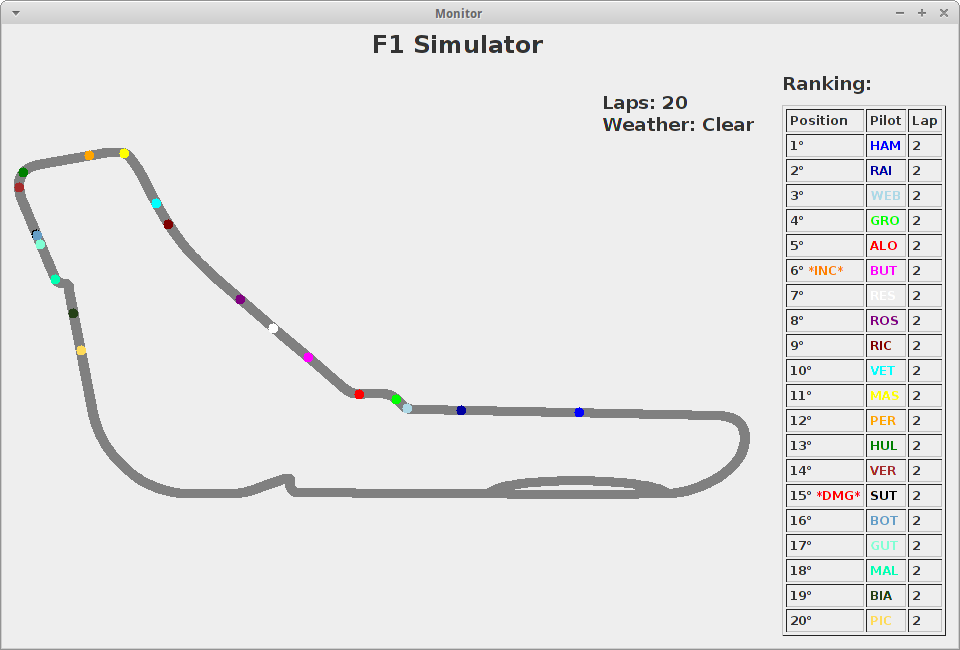
\includegraphics[keepaspectratio = true, width = 380px] {Pictures/monitor}
		\rule{35em}{0.5pt}
	\caption[Monitor]{Monitor: Rappresentazione della pista con classifica.}
	\label{fig:Monitor}
\end{figure}

Come anticipato, il monitor è l’elemento che permette all’utente di vedere in modo chiaro ed immediato l’andamento della gara.
Il monitor contiene due elementi fondamentali, la classifica (con gli stati attuali delle vetture) e la rappresentazione grafica dello stato della pista. Quest’ultima si basa sui dati ottenuti dal broker, ma non si limita a visualizzarli semplicemente a schermo, ma viene prima effettuata una seconda interpolazione per permettere di rendere fluida l’animazione del movimento dei veicoli.
Il setup del monitor reperisce informazioni da più fonti, infatti viene effettuato un pull di dati dal broker per il numero dei giri e di veicoli, mentre tutto quello che riguarda specifiche ulteriori (di visualizzazione) è contenuto nei file di configurazione. L’oggetto Drivers (Drivers.java) si occupa di leggere i dati contenuti nel file “carsProp.txt”, in cui sono contenute le informazioni riguardanti i nomi dei piloti ed il colore del loro veicolo. Abbiamo scelto di mantenere queste informazioni separate dal core perché non sono necessarie al funzionamento del simulatore, e avrebbero implicato un numero maggiore di informazioni da inviare tra i vari nodi del sistema distribuito. Inoltre in questo modo l’utente può personalizzare i colori ed i nomi dei piloti che vengono visualizzate sul monitor di cui dispone.
Successivamente deve essere letta e creata la pista; il file che viene utilizzato dal core per la creazione dei segmenti non è sufficiente, dato che include solo i dati necessari alla simulazione fisica, ma non spiega la forma del tracciato. Per questo motivo il file contenente la mappa del circuito è separato. Ogni segmento del circuito viene rappresentato come un oggetto con interfaccia Segment (Segment.java), che è stato implementato da due classi, StraightSegment e TurnSegment. Come intuibile dal nome il primo rappresenta un segmento rettilineo, mentre il secondo una curva. Ogni Segment offre la funzione getPosition, che data la percentuale di avanzamento del segmento restituisce la posizione in pixel in cui è presente il veicolo. Per quanto la funzione sia la stessa per i due tipi di segmento, la loro implementazione è profondamente diversa.
I segmenti rettilinei vengono inizializzati tramite quattro variabili intere, che rappresentano relativamente il punto di inizio del segmento ed il punto di fine. Data la percentuale di percorrenza, è facile utilizzare una proporzione in centesimi per ricavare la posizione corrente all’interno del tratto.
La situazione è differente per le curve, infatti abbiamo dovuto cercare un metodo per rappresentarle che fosse preciso, flessibile, ed impostabile manualmente (per permettere ad un utente di creare il proprio circuito). La prima idea è stata quella di definire solo alcuni tipi di curve possibili, e collegarle con i segmenti, in modo da assemblare la pista con una serie di “pezzi” possibili. Il problema di questa soluzione è che inevitabilmente avrebbe tolto la possibilità di riprodurre un tracciato reale esistente, caratteristica piuttosto importante per ogni appassionato di F1.
Quindi abbiamo cercato un modo per rendere la rappresentazione più fedele alla realtà, e di conseguenza abbiamo cercato di affidarci a formule matematiche ad hoc per ogni curva, ma come è facilmente intuibile questa soluzione è tutt’altro che pratica per la costruzione manuale di un tracciato.
La soluzione che abbiamo adottato, è quella che viene spesso utilizzata nei software di computer grafica, cioè l’utilizzo delle curve di Bézier; queste curve parametriche vengono definite da un numero variabile di punti intermedi, che ne specificano la concavità. Nel nostro caso abbiamo utilizzato delle curve cubiche, cioè caratterizzate da quattro punti (gli estremi e due ulteriori punti di controllo).
Una volta ottenuti tutti i dati sui segmenti, un oggetto di tipo Drawer (Drawer.java) percorre virtualmente ogni punto disponibile, disegnando l’immagine della pista; questa immagine verrà poi utilizzata come sfondo del pannello su cui verranno rappresentati i veicoli.
Successivamente viene effettuata la registrazione al publisher del broker, istanziando un oggetto della classe Communicator.java; ogni aggiornamento inviato dal broker viene ricevuto da quest’ultimo, che aggiorna un oggetto Container, che contiene tutte le informazioni necessarie alla rappresentazione della gara. L’oggetto Container si può considerare come il “magazzino” in cui vengono salvati gli ultimi dati ricevuti, e data l’elevata frequenza di aggiornamenti, è piuttosto probabile che si verifichi la situazione in cui vengono scritti i dati finché la rappresentazione è in corso. Per questo motivo entrambi i metodi necessari all’accesso (set e get) sono stati resi mutuamente esclusivi, cioè di fatto il Container è stato reso una risorsa protetta. 
Il Communicator non ha solo il compito di ricevere le informazioni e salvarle, infatti è proprio questa classe che implementa l’interpolazione dei dati ricevuti. Dato che il tempo che trascorre tra due ricezioni è noto ed impostato manualmente (500 ms), è stata creata una sequenza di dieci peridodi transitori di 50 ms l’uno, in cui si avanza di 1/10 della differenza tra il nuovo stato ed il vecchio. In questo modo è come ricevere uno snapshot ogni 50 ms invece che ogni 500, aumentado i frame al secondo da 2 a 20, che permettono l’illusione di un movimento continuo.
Può sembrare strano aver effettuato due interpolazioni, una sul broker ed una sul monitor, ma la scelta non è stata casuale. Le due interpolazioni hanno un significato molto diverso tra loro, infatti quella presente nel broker ha il compito di trasformare i dati, e farli passare dal dominio dello spazio a quello del tempo, con una complessità non indifferente ed utilizzando della conoscenza su come è stato costruito il core. La seconda invece, ha il solo scopo di rendere la rappresentazione grafica più gradevole per l’utente, riducendo le distanze tra due step successivi, senza considerare ulteriori informazioni; inoltre inviando questi dati tramite messaggi, avremmo strettamente legato l’avanzamento della rappresentazione alla latenza della rete, particolare non trascurabile.
Per questo a nostro avviso la scelta più sensata è stata quella di dividere completamente l’elaborazione dei dati per la simulazione dall’elaborazione con fini grafici.
L’ultimo oggetto istanziato dal monitor è quello che effettivamente ne permette la visualizzazione, cioè la finestra ed il relativo contenuto, presente nella classe Window.java.
Dato che i dati sono stati gestiti precedentemente, il lavoro dell’oggetto Window si limita ad ordinare per posizione i veicoli, rappresentarli graficamente tramite lo stesso Drawer utilizzato per la costruzione della pista, e disegnare una classifica (tramite tabella in HTML) con i nomi dei piloti ed il loro stato. Il refresh viene effettuato ogni 50 ms, in modo da utilizzare tutti gli snapshot ottenuti tramite l’interpolazione.
Come anticipato nei precedenti capitoli, per scelta progettuale la finestra non si chiuderà alla conclusione della gara, e la terminazione di questo nodo è basata solo sulla chiusura della finestra collegata, che orchestra la fine di ogni thread attivo.
Tutti i vari step del monitor, dal setup alla chiusura, sono completamente indipendenti dallo stato della gara, infatti è possibile collegare questo nodo in qualsiasi momento, dato che in ogni publish del broker vengono inviate tutte le informazioni necessarie alla completa rappresentazione della gara.

\subsection{Controller}

\begin{figure}[htbp]
	\centering
		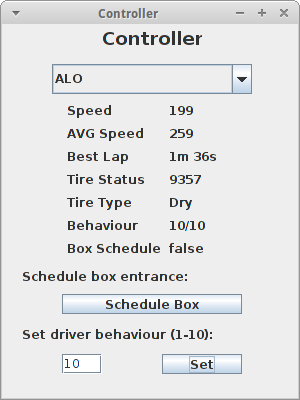
\includegraphics[keepaspectratio = true, width = 200px] {Pictures/controller}
		\rule{35em}{0.5pt}
	\caption[Controller]{Controller: Dati aggiuntivi e strumenti per modificare alcuni parametri.}
	\label{fig:Controller}
\end{figure}

Il controller è l’elemento che permette all’utente di interagire con l’andamento della gara. L’idea di base è quella di fornire un controllo simile a quello che possono avere i box, e quindi restare su un livello prettamente strategico.
Siccome è impensabile far fare scelte che richiedano tempi di risposta troppo veloci ad un giocatore inesperto, abbiamo deciso di fornire all’utente solamente la possibilità di manipolare decisioni che abbiano valenza anche se vengono prese in considerazione dopo un breve tempo di attesa.
L’idea alla base dell’implementazione del controller è abbastanza simile a quella del monitor, anche se è semplificata dal fatto di non avere i vincoli di refresh necessari alla rappresentazione.
Come prima cosa, viene richiesto il setup al broker, passo necessario per ottenere le informazioni sul numero di veicoli partecipanti. Come per il monitor, i veicoli vengono identificati nei messaggi solo da un numero, e la loro traduzione con il nome del pilota viene effettuata tramite lo stesso file utilizzato dal monitor per la classifica.
Dato il diverso tipo di comunicazione è stata implementata una nuova classe per la sua gestione, chiamata ControllerCommunicator.java. Questa classe è profondamente diversa da quella vista precedentemente nel monitor, infatti i dati non vengono più ricevuti in subscribe dal broker, ma devono essere richiesti (pull); questo implica che non è più una entità attiva che raccoglie i dati, ma diventa un’entità passiva che invia richieste solo quando necessario.
Il suo compito non si limita a fare richieste in pull tramite il metodo “getDetail”, ma comprende anche l’invio dei messaggi di override al core, tramite i metodi “overrideBehaviour” e “overrideBoxEntrance”.
Successivamente viene inizializzato un oggetto della classe ControllerWindow.java, che contiene il pannello della finestra, su cui vengono mostrate le varie informazioni.
Nella finestra è possibile scegliere un veicolo dalla lista, e da quel momento verranno visualizzati i dettagli relativi alla macchina, e ogni istruzione inviata si riferirà a quella specifica vettura.
Al termine della gara la finestrà non si chiude, ma avvisa l’utente che la connessione è stata interrotta; solo alla chiusura della finestra viene chiuso definitivamente il controller.
Come per il monitor, l’avvio e la relativa connessione possono essere effettuati in qualsiasi momento, non necessariamente all’avvio della gara.

\subsection{Eventi}

Come già accennato precedentemente, la simulazione nel core generea un flusso continuo di eventi che vengono poi inviati all’intermediario. Gli eventi sono composti da un numero variabile di coppie chiave-valore, diverse per ogni tipo. Vediamo ora in dettaglio la loro composizione:

Fine Segmento: \\
   type = ES $|$ car = (Pos)ID $|$ seg = (Pos)Seg\textunderscore ID $|$ vel = (Int)speed $|$ beh = (Pos)behaviour $|$
   tire\textunderscore s = (Int) tire\textunderscore status $|$ tire\textunderscore t = (bool)rain\textunderscore tire $|$ time = (time\textunderscore span) $|$ r\textunderscore box =(bool)request\textunderscore box

Rientro ai box: \\
   type = EB $|$ car = (Pos)ID $|$ time = (time\textunderscore span)

Uscita dai box: \\
  type = LB $|$ car = (Pos)ID $|$ tire\textunderscore t = (bool)rain\textunderscore tire $|$ lap = (Pos)giro terminato $|$ time = (time\textunderscore span)

Fine Giro: \\
  type = EL $|$ car = (Pos)ID $|$ lap = (Pos)giro terminato $|$ time = (time\textunderscore span)

Una macchina conclude la gara: \\
  type = CE $|$ car = (Pos)ID $|$ time = (time\textunderscore span)

La gara è finita: \\
  type = ER

Una macchina fa un incidente: \\
  type = CA $|$ car = (Pos)ID $|$ damage = (bool) $|$ retired = (bool) $|$ seg = (Pos)segmento $|$
  time = (time\textunderscore span)

Cambio meteo: \\
   type = WC $|$ rain = (bool)

Setup: \\
  type = SE $|$ ncar = (Int)real\textunderscore car\textunderscore number $|$ nlap = (int)real\textunderscore laps\textunderscore number
  
\subsection{Snapshot}

Gli eventi sopracitati, vengono tradotti dall’intermediario in uno snapshot, ovvero una fotografia dello stato della gara in un dato istante. Come già detto, ce ne sono di due tipi: lo snapshot generalista e quello dettagliato.
Lo snapshot generalista contiene una riga per ogni macchina, ed è composta da:

\begin{itemize}
 \item lap(Integer) = numero di giro di pista corrente
 \item segment(Integer) = identificativo del segmeno in cui è correntemente (-1 per il box)
 \item progress(Float) = percentuale di completamento del segmento corrente
 \item incident(Boolean) = indica che sta facendo un incidente, è fuori pista
 \item damaged(Boolean) = indica se è danneggiata
 \item retired(Boolean) = indica se si è ritirata
 \item over(Boolean) = indica se ha finito la corsa
 \item ranking(Integer) = indica la sua posizione in classifica
\end{itemize}

Nello snapshot dettagliato troviamo invece, per ogni macchina:

\begin{itemize}
 \item tire\textunderscore status(Integer) = livello degli pneumatici
 \item rain\textunderscore tires(Boolean) = indica se monta gomme da pioggia
 \item average\textunderscore speed(Float) = la media di velocità tenuta da inizio corsa
 \item behaviour(Integer) = il comportamento che tiene il pilota, da 1 a 10
 \item current\textunderscore speed(Integer) = la velocità attuale
 \item require\textunderscore box(Boolean) = indica se ha richiesto una sosta ai box
\end{itemize} 
% Chapter Template

\chapter{Copertura dei requisiti} % Main chapter title

\label{Chapter7} % Change X to a consecutive number; for referencing this chapter elsewhere, use \ref{ChapterX}

\lhead{Capitolo 7. \emph{Copertura dei requisiti}} % Change X to a consecutive number; this is for the header on each page - perhaps a shortened title

I requisiti del sistema erano:

\begin{itemize}
 \item 1) un circuito, possibilmente selezionabile in fase di configurazione, dotato almeno della pista e della corsia di rifornimento, ciascuna della quali soggette a regole congruenti di accesso, condivisione, tempo di percorrenza, condizioni atmosferiche, ecc.
 \item 2) un insieme configurabile di concorrenti, ciascuno con caratteristiche specifiche di prestazione, risorse, strategia di gara, ecc.
 \item 3) un sistema di controllo capace di riportare costantemente, consistentemente e separatamente, lo stato della competizione, le migliori prestazioni (sul giro, per sezione di circuito) e anche la situazione di ciascun concorrente rispetto a specifici parametri tecnici
 \item 4) una particolare competizione, con specifica configurabile della durata e controllo di terminazione dei concorrenti a fine gara.
\end{itemize}

Il punto 1 è soddisfatto perchè il circuito di gara viene letto durante l’avvio del sistema da file testuali e costruito in modo da avere sempre una corsia di rifornimento (box). All’interno dei suddetti file sono definite le regole di accesso per ogni segmento che ne fa parte, oltre ad informazioni riguardanti la lunghezza o la difficoltà che permettono al simulatore di calcolarne coerentemente il tempo di percorrenza. Il tempo atmosferico viene gestito da un entità attiva separata dal resto del sistema, e cambia in modo completamente casuale.
Per quanto riguarda il punto 2, abbiamo che l’insieme dei concorrenti è memorizzato anch’esso all’interno di un file testuale. Ogni concorrente ha le proprie specifiche caratteristiche di velocità massima, accelerazione e comportamento tenuto in gara memorizzate all’interno di tale file.
Il punto 3 viene soddisfatto dal monitor, in grado di riportare lo stato della competizione, e dal controller, in grado di mostrare per il pilota selezionato le migliori prestazioni sul giro e altri parametri utili per decidere la strategia.
Infine, per il punto 4, abbiamo che durata e numero di partecipanti alla competizioni vengono anch’essi letti da un file testuale, e al termine gara abbiamo una chiusura ordinata dei componenti facente parte del sistema. 
% Chapter Template

\chapter{Conoscenze apprese} % Main chapter title

\label{Chapter8} % Change X to a consecutive number; for referencing this chapter elsewhere, use \ref{ChapterX}

\lhead{Capitolo 8. \emph{Conoscenze apprese}} % Change X to a consecutive number; this is for the header on each page - perhaps a shortened title

Ciò che abbiamo imparato in questo corso non riguarda solamente la materia proposta, infatti la più grande differenza rispetto ad ogni altro corso (riferito alla nostra esperienza personale) è data dalla fase di progettazione. Solitamente dato un certo obiettivo, il fine era solamente quello di costruirne un prototipo funzionante, non preoccupandosi eccessivamente della correttezza delle scelte, ma cercando di adattarle progredendo nello sviluppo; in questo caso invece, ci siamo trovati in una condizione nuova, in cui la parte di programmazione non viene preposta al resto, ma diventa secondaria alla progettazione e alla risoluzione concettuale delle problematiche. 
Questo approccio ha mostrato i suoi frutti appena è stato necessario mettere in pratica ed implementare le idee maturate durante la progettazione, infatti, tralasciando le problematiche intrinseche all’uso di un linguaggio per noi nuovo, non è stato necessario inventare soluzioni nuove, ma seguire il percorso costruito precedentemente. Questo ha comportato anche un numero considerevolmente inferiore di problemi causati da effetti collaterali di soluzioni non pensate adeguatamente, facilitando la fase di implementazione.
Un’altra cosa che riteniamo molto importante è ciò che il corso (ed il relativo progetto) ci ha insegnato riguardo alla concorrenza, e l’importanza di costruire un’architettura robusta in grado di mantenere un comportamento coerente anche con l’uso di più task e risorse condivise, cosa sicuramente non banale e che causa problemi ed errori difficilmente individuabili. Proprio riguardo questa parte è stato importante capire come la scelta del linguaggio non sia basata sulla semplicità di quest’ultimo, ma dipenda dall’utilizzo e dai vincoli necessari al funzionamento del programma: utilizzare Java al posto di Ada nelle situazioni critiche del core o del broker avrebbe reso complicato se non impossibile garantire la correttezza dell’esecuzione ed il suo determinismo logico, facilmente ottenibile tramite le entry e procedure di cui dispone Ada.
Altra cosa importante è ciò che abbiamo imparato riguardo la distribuzione, solitamente affrontata manualmente tramite socket o altri espedienti. In un sistema complesso risulta importante poter definire a priori l’architettura su cui si basa l’intero sistema, in modo da essere a conoscenza di ciò che accade tra ogni nodo. Per quanto nel nostro caso non sia stato utilizzato un middleware, bensì una libreria per lo scambio di messaggi, abbiamo comunque definito gli attori del nostro sistema durante la progettazione, ma come detto precedentemente abbiamo scelto di non legarci ad un altro software per mantenere la portabilità del codice, e quindi abbiamo optato per una soluzione che si pone in mezzo tra la rigidità del middleware e la flessibilità (e relativa fragilità) dell’implementazione manuale.  
% Chapter Template

\chapter{Configurazione ed utilizzo} % Main chapter title

\label{Chapter9} % Change X to a consecutive number; for referencing this chapter elsewhere, use \ref{ChapterX}

\lhead{Capitolo 9. \emph{Configurazione ed utilizzo}} % Change X to a consecutive number; this is for the header on each page - perhaps a shortened title

La configurazione dei parametri della simulazione viene effettuata tramite cinque file di testo.
Il file race\textunderscore properties.txt contiene solamente due elementi, il numero di giri ed il numero di veicoli, separati da uno spazio.
Nel file cars.txt sono presenti tutte le caratteristiche di ogni veicolo, una macchina per ogni riga; in ordine vanno definiti ID, comportamento di default (da 1 a 10), velocità massima in $Km/h$, ed accelerazione in $m/s^2$. Il numero massimo di macchine ammissibile è 20.
Il circuito logico (cioè i dati utilizzati nella simulazione e non nella visualizzazione) sono contenuti nel file circuit.txt, in cui in ogni riga va inserito un singolo segmento. Le proprietà di ogni segmento sono: ID, lunghezza in metri, molteplicità di vetture contenute, difficoltà, ed un flag t/f che indica se è presente l’ingresso ai box.
Durante la costruzione il programma collegherà automaticamente ogni segmento al successivo, e l’ultimo segmento al primo, in modo da creare un circuito chiuso.
I file visti finora sono utilizzati per la logica del sistema, mentre i due successivi per la visualizzazione nel monitor.
CarsProp.txt permette l’associazione dell’ID di ogni veicolo ad un soprannome (tipicamente le prime tre lettere del cognome) ed a un colore. All’interno del file il numero di riga indica l’ID del veicolo associato.
L’ultimo file è quello che contiene le informazioni necessarie alla visualizzazione del circuito; circuitMap.txt deve contenere come prima riga un solo numero, che indica il numero di segmenti totali. Successivamente ogni riga rappresenta un tratto, che può essere di due tipi: ogni rettilineo ha come primo valore il carattere ‘S’, seguito dalle coordinate x e y dei punti di inizio e fine, mentre ogni curva ha come primo valore il carattere ‘T’ seguito dai punti necessari alla costruzione della curva di Bézier. Un caso particolare è il tratto del box, caratterizzato dal carattere ‘B’ e trattato come una curva, il cui ingresso è fissato al termine del penultimo segmento e l’uscita è al quarto.
Tramite questi file è possibile modificare ogni caratteristica della simulazione, dai piloti al circuito, avendo la possibilità di ricostruire una gara a piacere.
La seconda configurazione necessaria è quella della distribuzione, infatti ogni nodo del sistema ha diversi requisiti. All’avvio di ogni componente è necessario specificare come parametri da linea di comando gli indirizzi di cui ha bisogno, cioè i seguenti:

\begin{itemize}
 \item Broker:
 \begin{itemize}
  \item [1] Indirizzo locale su cui ricevere i dati del core
  \item [2] Indirizzo locale su cui avviare il publisher per le comunicazioni al monitor
  \item [3] Indirizzo e porta locale su cui avviare il server necessario al pull
 \end{itemize}
 \item Core (main):
 \begin{itemize}
  \item [1] Indirizzo del broker ([1] del broker)
  \item [2] Indirizzo locale su cui avviare il server in ascolto per il controller
 \end{itemize}
 \item Monitor:
 \begin{itemize}
  \item [1] Indirizzo per il subscribe al broker ([2] del broker)
  \item [2] Indirizzo per il pull dal broker ([3] del broker)
 \end{itemize}
 \item Controller:
 \begin{itemize}
  \item [1] Indirizzo per il pull dal broker ([3] del broker)
  \item [2] Indirizzo del core a cui inviare gli override ([2] del core)
 \end{itemize}
\end{itemize}

Inoltre è presente un solo vincolo di avvio, cioè il broker deve essere avviato prima del core; il monitor ed il controller invece possono essere avviati in qualsiasi momento.
Dato il grande numero di parametri, è stato creato nella cartella “scd-f1-simulator” un eseguibile start.sh, che avvia le varie parti in modo che eseguano su un solo computer. 

%----------------------------------------------------------------------------------------
%	THESIS CONTENT - APPENDICES
%----------------------------------------------------------------------------------------

%\addtocontents{toc}{\vspace{2em}} % Add a gap in the Contents, for aesthetics

%\appendix % Cue to tell LaTeX that the following 'chapters' are Appendices

% Include the appendices of the thesis as separate files from the Appendices folder
% Uncomment the lines as you write the Appendices

%% Appendix A

\chapter{Appendix Title Here} % Main appendix title

\label{AppendixA} % For referencing this appendix elsewhere, use \ref{AppendixA}

\lhead{Appendix A. \emph{Appendix Title Here}} % This is for the header on each page - perhaps a shortened title

Write your Appendix content here.
%\input{Appendices/AppendixB}
%\input{Appendices/AppendixC}

%\addtocontents{toc}{\vspace{2em}} % Add a gap in the Contents, for aesthetics

\backmatter

%----------------------------------------------------------------------------------------
%	BIBLIOGRAPHY
%----------------------------------------------------------------------------------------

%\label{Bibliography}

%\lhead{\emph{Bibliography}} % Change the page header to say "Bibliography"

%\bibliographystyle{unsrtnat} % Use the "unsrtnat" BibTeX style for formatting the Bibliography

%\bibliography{Bibliography} % The references (bibliography) information are stored in the file named "Bibliography.bib"

\end{document}  